% !TeX root = RJwrapper.tex
\title{LBBNN: An R Package for Sparse and Explainable Bayesian Deep Learning with Latent Binary Bayesian Neural Networks}
\author{by Lars Skaaret-Lund, Eirik Høyheim and Aliaksandr Hubin }

\maketitle

%abstract maximum 150 words
\abstract{
The package LBBNN (latent binary Bayesian neural networks) provides a framework for doing sparse uncertainty aware and to a large degree interpretable Bayesian inference in neural network models, with potentially huge datasets, and highly overparametrized networks. Currently, most packages implementing Bayesian neural networks in R use Markov chain Monte Carlo based inference, without the possibility of GPU acceleration. Our package, using variational inference and the LibTorch backend (via the \code{torch} package), provides a more scalable and computationally efficient approach. The package integrates three different methodological works: Firstly, it takes into account the basic LBBNN model, where each weight in the network is associated with a Bernoulli latent inclusion indicator, allowing for incorporating model uncertainty and achieving substantial sparsification of the network while maintaining high predictive power. Secondly, using normalizing flows allows for modeling more complex and flexible variational distributions with statistical dependencies. And thirdly, by allowing the input variables to skip to any layer in the network, we can model different types of functions, e.g. we might only have linear connections. This allows for more explainable results. Lastly, local explanations at the prediction level with uncertainty are provided in the LBBNN package and are guaranteed to be exact for piecewise linear activations.  To demonstrate how the package can be used in practice, we include experiments on both synthetic data and real-world datasets, covering both tabular and image based data.
}

\section{Introduction}
Modern deep learning architectures are typically parameterized by billions of parameters, in addition to being black box, and not offering uncertainty quantification, which makes them problematic to use in highly sensitive domains. Bayesian neural networks (BNN) alleviate the latter issue by having uncertainty quantification easily accessible by treating the model parameters as random variables. Further, the development of Latent Binary Bayesian Neural Networks (LBBNN) \citep{hubin2024sparse} allows for a scalable Bayesian approach to sparse neural network learning, by including a Bernoulli inclusion indicator variable for each weight. This allows using model uncertainty to reduce a network to a fraction of its initial size, while maintaining all the other advantages of doing Bayesian inference. In the frequentist setting, sparsification is usually obtained by more ad hoc procedures (see e.g. \cite{frankle2018lottery}).

Two limitations of LBBNNs as defined in \cite{hubin2024sparse} are addressed in \cite{skaaret-lund2024sparsifying}. The first is that while LBBNNs are sparser than BNNs during inference, they are still computationally expensive during training, since one has to sample \emph{two} large matrices, one for the weights and one for the inclusion parameters for each layer in the network during forward propagation. The second issue is the mean-field posterior, which can only model the weights as independent random variables. The first issue is improved on by utilizing the local reparametrization trick (LRT) \citep{kingma2015variational}, which makes it possible to sample the (approximate) Gaussian activations directly, rather than the weights and the inclusion variables. Secondly, by including normalizing flows \citep{rezende2015variational}, the variational distribution can model more complex (and dependent) distributions instead of the simple mean-field Gaussian. However, this comes at the cost of having the additional flow parameters to optimize. 

In addition to the aforementioned LBBNN models, the package also aims to include perhaps the most important recent development, namely input-skip LBBNNs \citep{hoyheim2026explainable}. Input-skip refers to the design of a network such that the input is concatenated at each hidden layer. This, in addition to inclusion variables for these inputs, results in a network which could potentially include only linear functions, when the only non-zero inclusion variables will be from the inputs that have been concatenated at the last hidden layer, whereas standard networks must include all hidden layers. This is potentially very powerful, as traditional learning methods typically rely on selecting the model a priori, whereas in this case we can let the data decide the type of function to learn. In \cite{hoyheim2026explainable}, an experiment with synthetic data demonstrates the ability to select the correct function based on the data. The experiment shows that even though we start off dense (i.e. all connections from all layers are included), the network reduces to a simple linear function when the data is generated that way, or a more complicated non-linear one when that is required. In addition, input-skip LBBNNs also generally give even sparser networks than standard LBBNNs on standard benchmark datasets such as MNIST. Finally, input-skip LBBNNs also introduce a novel approach to obtaining global and local explanations of predictions, important in domains where understanding the contributions of individual variables is desirable. 

The latest stable release of the package can be installed from CRAN in an R session by running \code{install.packages("LBBNN")}.
%\textcolor{blue}{Give overview of existing R and python  libraries for sparse Bayesian deep learning (if any).}
%\textcolor{blue}{Write something here about the experiments and/or tutorials that will be included later.}

\section{Related work}
Bayesian neural networks have been around since the early 1990s. They were popularized by \cite{neal1995bayesian} in his PhD-thesis, where inference was done using Hamiltonian Monte Carlo (HMC) \citep{duane1987hybrid} to sample from the posterior distribution of the neural network weights. HMC is considered an improvement on traditional MCMC techniques, as it uses Hamiltonian dynamics to explore the parameter space more efficiently. However, HMC does not scale well with large datasets, and very high-dimensional parameter spaces such as neural network posteriors, as we typically see in modern applications. In addition, deep and overparameterized neural network posteriors are typically highly multi-modal, another area where HMC struggles.  

An alternative method that is more scalable is Variational Inference (VI) \citep{jordan1999introduction}. Rather than trying to sample from the true posterior distribution, VI defines a parameterized approximate posterior distribution, $q$, where the goal is to adjust the parameters of $q$ to minimize the discrepancy from the true posterior distribution, where the latter is typically measured by the KL-divergence. This optimization based approach is often preferred in practice (given finite computational budget) over HMC's asymptotically exact posterior samples, as one can utilize stochastic gradient descent and mini-batching of the data, using high performance parallel computing on modern GPU devices. Additionally, the objective function of VI is easy to monitor, avoiding the challenges of assessing HMC convergence in multi-modal settings. 

Recent work on scalable VI such as Improved Variational Online Newton (IVON) \citep{shen2024variational} uses an implicit mean-field Gaussian approximation over the weights, where the mean and variance are updated with online second order curvature estimates of the loss, achieving a computational cost comparable to Adam, enabling scaling to large neural network architectures. While such methods improve the scalability of variational inference, recent work has also focused on improvements in sampling based inference, such as Microcanonical Langevin Ensembles (MILE) \citep{sommer2025microcanonicallangevinensemblesadvancing}, which uses deep ensembles to initialize short MCLMC \citep{robnik2023fluctuation} chains. This achieves substantial computational gains over the No-U-Turn Sampler (NUTS) \citep{hoffman2014no} algorithm, at the cost of no longer guaranteeing asymptotic exactness of posterior sampling due to (deliberately) omitting the Metropolis step to correct the discretization bias.

Today, Python is the dominant programming language when implementing Bayesian (deep) neural networks. This is due to the availability of deep learning frameworks such as PyTorch \citep{paszke2019pytorch} and TensorFlow \citep{tensorflow2015-whitepaper}, providing key features like high performance GPU computation and automatic differentiation. While it is possible to implement Bayesian neural networks directly using these frameworks, both ecosystems provide probabilistic programming libraries such as Pyro \citep{bingham2019pyro} (for PyTorch) and TensorFlow Probability \citep{dillon2017tensorflow} which facilitate Bayesian modeling by providing abstractions for probabilistic models and inference algorithms. 

More recently, the Python ecosystem has grown to include \code{BlackJAX} \citep{cabezas2024blackjax}, providing efficient, accelerator-agnostic implementations of MCMC algorithms including NUTS and HMC. In addition, the \code{bde} \citep{arvanitis2026bde} library combines scikit-learn compatibility with JAX-based training and uncertainty quantification for Bayesian deep ensembles, in particular an implementation of MILE. Another approach is the \code{posteriors} package \citep{duffield2024scalable}, providing scalable Bayesian deep learning built directly on top of PyTorch.

While the above mentioned Python based tools can be accessed in R via the \code{reticulate} \citep{reticulate} package, this requires a properly configured Python/PyTorch environment alongside the R environment, which can introduce additional installation and dependency management considerations. In contrast, the R native \code{torch} \citep{torchR} package builds directly on libtorch, the backend C++ library that also powers PyTorch.

To the best of our knowledge, there is no R package that provides BNNs built on top of \code{torch}. The only R package we could find that offers GPU-accelerated variational inference for BNNs is \code{BayesFluxR} \citep{bayesfluxr} (itself a wrapper around a Julia backend), while the others --- \code{bnns} \citep{bnns}, \code{BNN} \citep{liang2018bayesian}, \code{BLNN} \citep{sharaf2020blnn}, \code{BoomSpikeSlab}  \citep{boomspikeslab}, and \code{selectnn} \citep{mcinerney2025statistical} rely on some form of MCMC. For a detailed comparison of these packages, see Table \ref{table:Rpackages}. 

Building on this gap, our \code{LBBNN} package offers a user friendly implementation of sparse BNNs (LBBNN) in R, built natively on the \code{torch} package, incorporating input-skip connections and supporting efficient optimization on modern high-performance hardware.

\setlength{\tabcolsep}{3pt}  % reduce column spacing

{\scriptsize
\begin{table}[ht]
\centering
\caption{Comparing our package LBBNN to other R packages implementing Bayesian neural networks.}
\begin{tabularx}{\textwidth}{l X X X X}
\hline
\textbf{Package} & \textbf{Description} & \textbf{Backend} & 
\textbf{Inference} & \textbf{Hardware} \\
\hline

\texttt{LBBNN} & BNNs with input-skip &
LibTorch / C++ & 
VI + normalizing flows &
CPU + GPU\\

\texttt{bnns} & Multi-layer feed forward BNN &
Stan / rstan &
MCMC (NUTS/HMC) &
CPU \\

\texttt{BayesFluxR} & BNNs in Julia &
Julia (BayesFlux.jl + Flux.jl) &
MCMC, VI  &
CPU + GPU \\

\texttt{BNN} & One hidden layer BNN + shortcut connections &
C &
MCMC &
CPU \\

\texttt{BLNN} & One hidden layer BNN &
R &
MCMC (HMC/NUTS) &
CPU \\
\texttt{BoomSpikeSlab} & spike and slab regression &
R / C++ &
MCMC &
CPU \\
\texttt{selectnn} & Neural network model selection &
R  &
MLE + BIC &
CPU \\

\hline
\end{tabularx}
\label{table:Rpackages}
\end{table}
}

\section{Models}
Given input variables, $\boldsymbol{x} \in \mathbb{R}^n$, and a response variable $\boldsymbol{y} \in \mathbb{R}^m$, a neural network models their relationship through a probability distribution $f$ parameterized by the vector $\boldsymbol{\eta}(\boldsymbol{x})$,
\begin{equation*}
\begin{split}
    \boldsymbol{y} &\sim f(\cdot;\boldsymbol{\eta}(\boldsymbol{x})),
    \end{split}
\end{equation*}
 with $f$ being a suitable distribution, e.g. for binary classification, $\boldsymbol{\eta}_i$ would be a vector of probabilities of success for the Bernoulli distribution.
For LBBNNs, the vector of parameters $\boldsymbol{\eta}(\boldsymbol{x})$ is attained through a composition of semi-affine transformations:
\begin{equation}\label{eq:u.act}
    u_{j}^{(l)} = \sigma^{(l)}\bigg(\sum\limits_{i=1}^{n^{(l-1)}} u_i^{(l-1)}\gamma_{ij}^{(l)}w_{ij}^{(l)} + \gamma_j^{(l)}b_j^{(l)}\bigg), j = 1,\ldots,n^{(l)}, l = 1,\ldots,L,
\end{equation}
{where} $\eta_{j}(\boldsymbol{x}) = u_{j}^{(L)}$. Additionally, $\boldsymbol u^{(l-1)}$ are the inputs from the previous layer (with $\boldsymbol u^0=\boldsymbol x$). The $w_{ij}^{(l)}$'s are the weights and $b_j^{(l)}$'s  -- the bias terms. For each layer $l$ of a total $L$ layers, $n^{(l)}$ denotes the number of neurons,  with $n^{(0)} = n$ the number of input variables. Furthermore, we have elementwise non-linear activation functions $\sigma^{(l)}$.
Finally, $\gamma_{ij}^{(l)}$ and $\gamma_{j}^{(l)}\in\{0,1\}$ are the binary inclusion variables for their corresponding weights and bias respectively. When all $\gamma_{ij}^{(l)} =1$, equation \eqref{eq:u.act} reduces to a standard BNN. In this case, we typically use independent Gaussians for the prior distribution of the weights and biases: 
\begin{align}\label{eq:BNNprior}
    p(w_{ij}^{(l)}) &= \mathcal{N}(w_{ij};0,\sigma_w^{2(l)});\\
    p(b_j^{(l)}) &= \mathcal{N}(b_j^{(l)};0,\sigma_b^{2(l)}).
\end{align}
To take into account uncertainty in both weights, and the structure of the network, we use the spike-and-slab prior for our LBBNNs:
\begin{equation*}
    \begin{split}
    p(w^{(l)}_{ij}|\gamma^{(l)}_{ij}) &= \gamma^{(l)}_{ij}\mathcal{N}(w^{(l)}_{ij};0,\sigma_w^{2(l)})+(1 - \gamma^{(l)}_{ij})\delta(w^{(l)}_{ij}); \\
    p(\gamma^{(l)}_{ij}) &= \text{Bernoulli}(\gamma^{(l)}_{ij};\alpha_w^{(l)}),
    \end{split}
\end{equation*}
and similarly for the biases. In the above, $\delta(\cdot)$ is the Dirac delta function, considered zero everywhere except at 0, where it has a spike. $\sigma^2$'s and $\alpha$'s denote the prior variances and inclusion probabilities for the weights (or biases). In our implementation, we allow for different values across layers, but within each layer they all have the same value. This is done for convenience but it is not strictly necessary. In principle each weight in the neural network could have a different prior inclusion and variance parameter.

%The extension to input-skip is as follows:
%\begin{equation}\label{eq:u.act-skip}    %u_{j}^{(l)} = %\sigma^{(l)}\bigg(\sum\limits_{i=1}^{n^{(l%-1)}+n} u_i^{(l-%1)}\gamma_{ij}^{(l)}w_{ij}^{(l)} + %\gamma_j^{(l)} b_j^{(l)}\bigg), j = %1,\ldots,n^{(l)}, l = 1,\ldots,L,
%\end{equation}
Lastly, with input-skip connections enabled, we concatenate the input to the hidden layers as follows:
\begin{equation}
    \boldsymbol{u}^{(l-1)} = \left[u_1^{(l-1)},\dots,u_{n^{(l-1)}}^{(l-1)},x_0,\dots,x_n\right],l = 2,\dots,L.
\end{equation}
For a graphical illustration of the differences between these methods, see Figure \ref{fig:model_comparison}.

To implement the LBBNNs, we will follow \citet{skaaret-lund2024sparsifying} and use LRT and normalizing flows. LRT allows for faster computations during training and inference, but assumes independent Gaussian distributions for the weights. Normalizing flows allow us to learn more complex variational posterior distributions as they account for dependencies between weights within a layer. Normalizing flows are implemented with RNVP \citep{dinh2016density} with the numerical stable updates presented in \citet{kingma2016improved}. For a more detailed overview of computational costs related to both LRT and normalizing flows, please see Appendix A in \citet{skaaret-lund2024sparsifying}. 

\begin{figure}
    \centering
    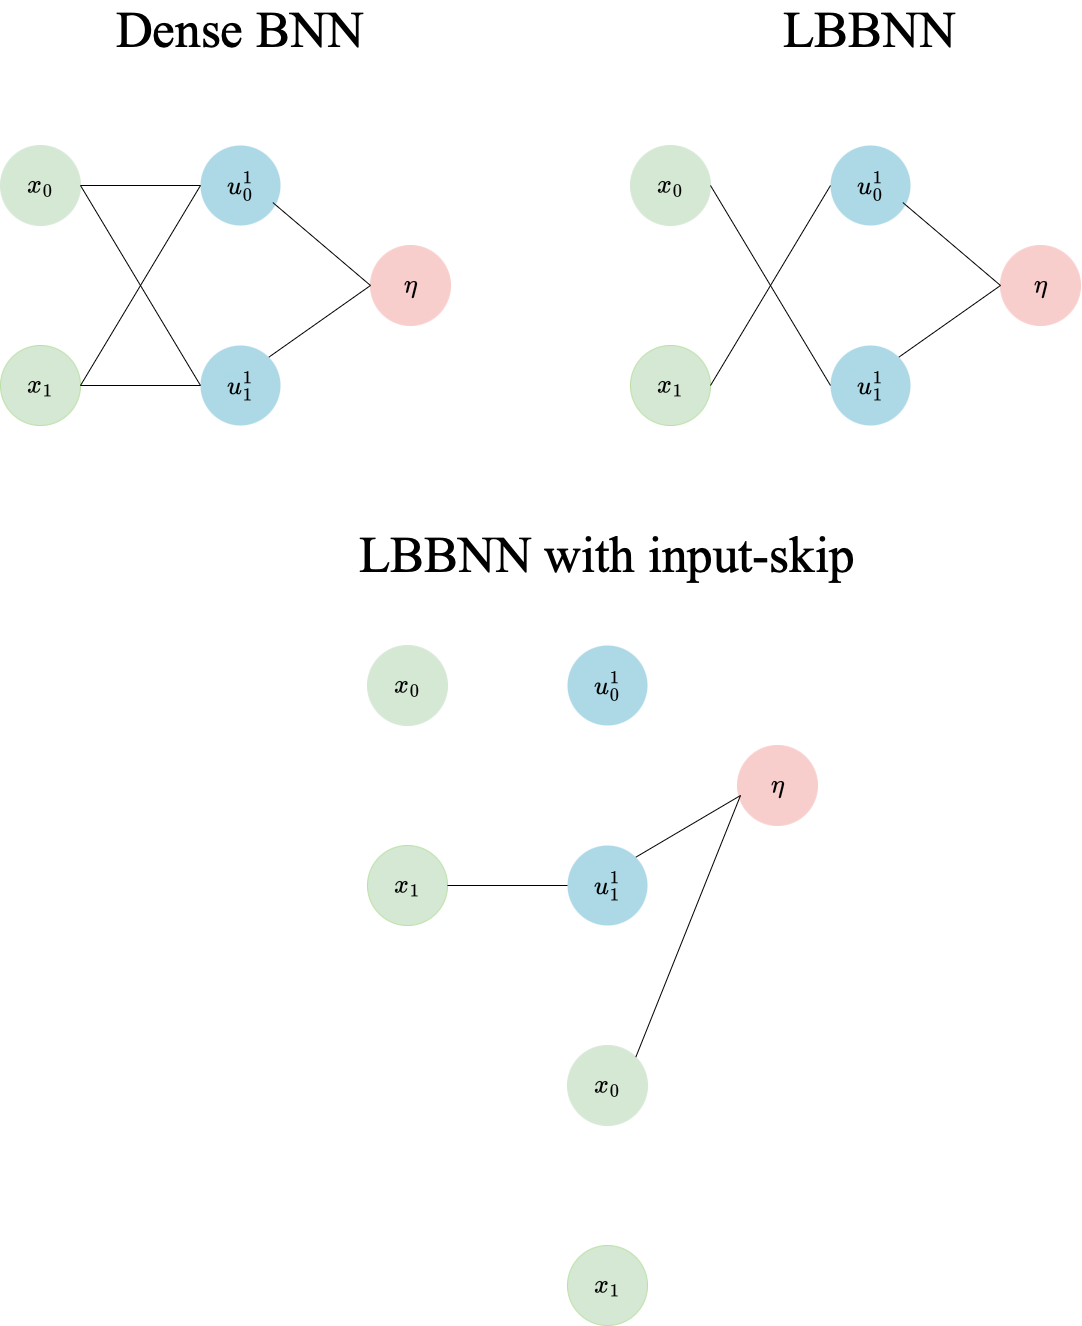
\includegraphics[width=.6\textwidth]
    {figures/diagram_R.png}
    \caption{Top left, a dense BNN where all connections are included. Top right, LBBNN where some connections have been removed, resulting in a sparser representation. Bottom, LBBNN with input-skip allows both a sparse representation, and having a linear connection between $x_1$ and the output.}
    \label{fig:model_comparison}
\end{figure}

\section{Package description}

\begin{figure}
    \centering
    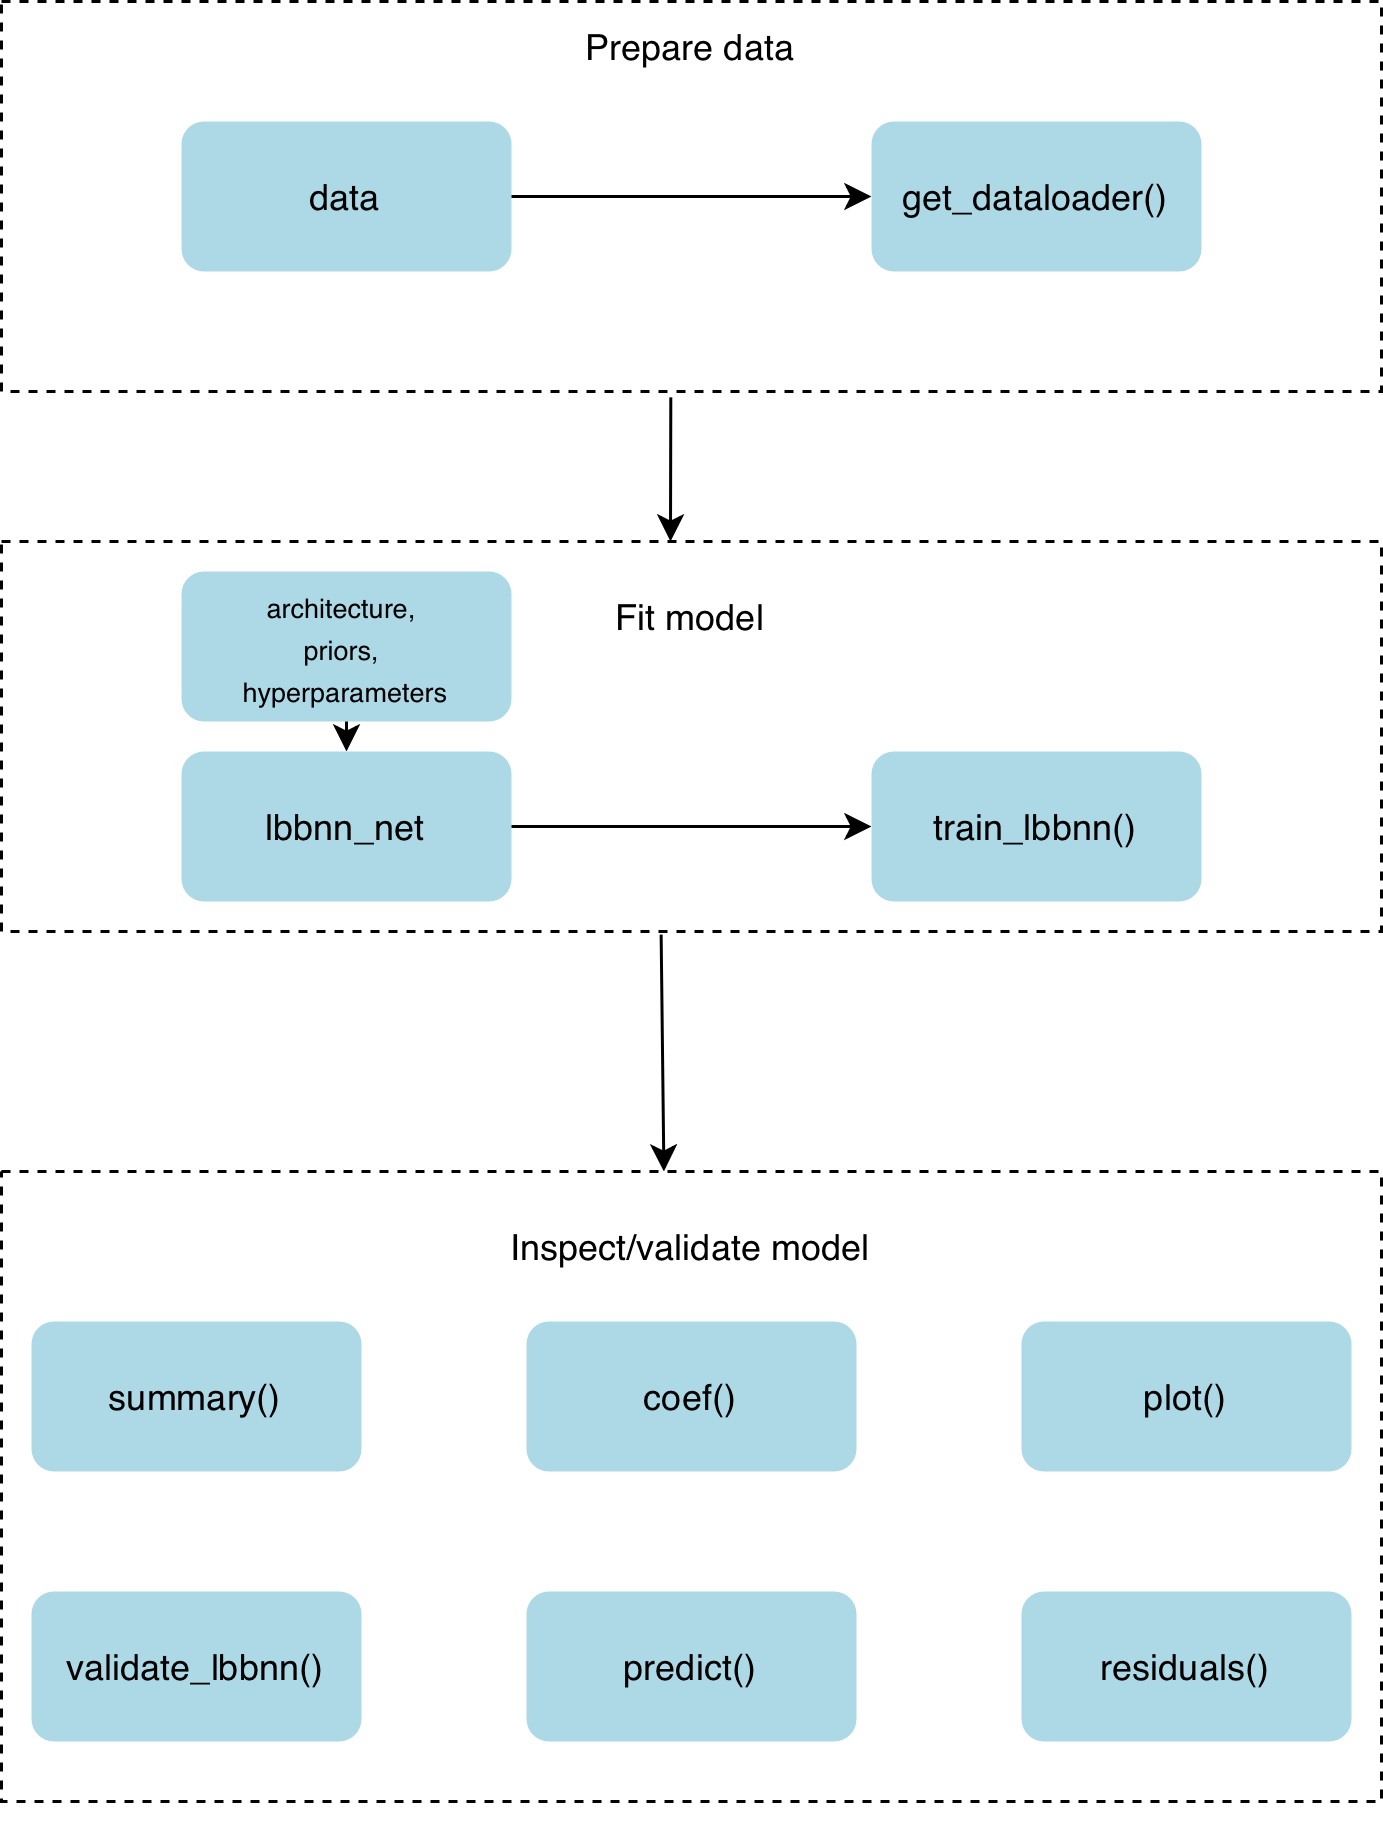
\includegraphics[width=.6\textwidth]
    {figures/package_diagram.png}
    \caption{Schematic overview of the package.}
    \label{fig:package_diagram}
\end{figure}

The main goal of LBBNN is to provide a framework to train Latent Binary Bayesian Neural Networks in R, using the \code{torch} package for high performance computation, while providing a user-friendly interface. For an overview of the workflow of the package, see Figure \ref{fig:package_diagram}. We implement many of the generic R functions such as \code{summary()}, \code{coef()} and \code{plot()} to facilitate clear and understandable output. These utility functions support both standard LBBNN architectures, and LBBNN with input-skip. We hope to make LBBNNs available for both statisticians and applied researchers, who work on problems where data might be high dimensional and non-linear in nature, and where the domain dictates that reliable uncertainty calibration and explainability is desirable. Below we demonstrate five detailed examples of how to use the package in practice. 

The first two deal with synthetic data, while the last three use real world data. The first tutorial is self-contained, whereas for the remaining tutorials we only report the most central details and refer the reader to the supplementary material for the full code needed to reproduce the examples.

\subsection{Tutorial 1: Simulation study with linear effects}
In the first example, we generate data in the following way:
\begin{align*}
    x_{ij}&\sim \mathcal{N}(0,1)\\ 
    y_i &= 0.6x_{i0}-0.4x_{i1} +0.5x_{i2} + \mathcal{N}(0,0.1),
\end{align*}
with $i = 1000$ and $j = 15$. The goal is to check if the model is able to remove the non-relevant variables, in addition to recovering the true linear effects. The data is generated as follows:
\begin{example}
library(LBBNN)
i <- 1000
j <- 15
set.seed(42)
torch::torch_manual_seed(42)
X <- matrix(rnorm(i * j, mean = 0, sd = 1), ncol = j)
y_base <-  0.6 * X[, 1] - 0.4 * X[, 2] + 0.5 * X[, 3] + rnorm(n = i, sd = 0.1)
sim_data <- as.data.frame(X)
sim_data <- cbind(sim_data, y_base)
\end{example}

\paragraph{Data preprocessing.} In \code{torch}, it is common to use \code{torch::dataloader} objects to automatically handle mini-batching\footnote{We will not give here an introduction to \code{torch} but rather refer the reader to detailed tutorials here \url{https://skeydan.github.io/Deep-Learning-and-Scientific-Computing-with-R-torch}.}, shuffling and parallel loading of the data when training the model. To avoid users having to interface directly with this, we provide a wrapper, the \code{get\_dataloaders()} function:
\begin{example}
loaders <- get_dataloaders(sim_data, train_proportion = 0.9,
                           train_batch_size = 450, test_batch_size = 100,
                           standardize = FALSE)
train_loader <- loaders$train_loader
test_loader  <- loaders$test_loader
\end{example}
The function returns one loader with training data and one with test data. In addition, \code{sim\_data} is a \code{data.frame} object with 1000 rows and 16 columns (the last being the target). In this example, we randomly select 900 samples for the training data, divided into two batches, and the remaining 100 as test samples. 

\paragraph{Model setup.} Further, we define the following hyperparameters:
\begin{example}
problem <- "regression"
sizes <- c(j, 5, 5, 1) # 2 hidden layers, 5 neurons in each
incl_priors <- c(0.5, 0.5, 0.5) #prior inclusion probability
stds <- c(1, 1, 1) #prior for the standard deviation of the weights
incl_inits <- matrix(rep(c(-10, 10), 3), nrow = 2, ncol = 3) #inclusion inits
device <- "cpu" #can also be 'gpu' or 'mps'
\end{example}
In the above, \code{incl\textunderscore inits} refers to the initialization of the parameters of the Bernoulli distribution governing weight inclusion, an important hyperparameter, as it controls the initial density of the network. In Tutorial 4, we go into more detail on different initialization strategies. The initial inclusion probabilities are computed with the logistic function, $\alpha_{\texttt{inits}} = \texttt{sigmoid(incl\_inits)}$, which in the example above will give inclusion probabilities between $4.54\cdot10^{-5}$ and $0.99995$. These hyperparameters are then used when defining an \code{lbbnn\textunderscore net} object:
\begin{example}
model_linear <- lbbnn_net(problem_type = problem, sizes = sizes,
                              prior = incl_priors, inclusion_inits = incl_inits,
                              std = stds, input_skip = TRUE, flow = FALSE,
                              num_transforms = 2, dims = c(10, 10, 10),
                              raw_output = FALSE, custom_act = NULL,
                              link = NULL, nll = NULL,
                              bias_inclusion_prob = FALSE, device = device)
\end{example}
The optional argument \code{input\_skip}
controls whether to use input\_skip. Further, \code{flow} is for using normalizing flows with variational inference, where \code{num\_transforms} and \code{dims} mean the number of transformations for the flow, and the dimensions of the hidden layers of the neural networks used in those transformations, respectively. \code{raw\_output} gives the outputs of the last layer before any sigmoid/softmax transformation. Additionally, \code{link} and \code{nll} are for the user to supply their own link and likelihood function. \code{bias\_inclusion\_prob} determines whether the bias parameters should be associated with inclusion indicators. Lastly, \code{device} gives the option to move the training process to either \code{mps} or \code{gpu} devices. 

\paragraph{Statistical inference.} For training, we use the function \code{train\textunderscore lbbnn}, where we pass the dataloader object defined earlier. In addition, \code{epochs} refers to the number of epochs to train for, where one epoch is a complete pass through the training dataset. \code{lr} defines the learning rate for the optimizer:
\begin{example}
train_lbbnn(epochs = 300, LBBNN = model_linear,
            lr = 0.05, train_dl = train_loader, device = device)
\end{example}
The training process can be monitored on the console:
\begin{example}
Epoch 1, training: loss = 827.28314, density = 0.47692 
Epoch 2, training: loss = 711.41266, density = 0.46667 
Epoch 3, training: loss = 618.56586, density = 0.46154 
...
Epoch 299, training: loss = 29.64363, density = 0.04615 
Epoch 300, training: loss = 29.75975, density = 0.04615 
\end{example}
Showing the loss and density (proportion of weights with inclusion probabilities greater than 0.5) at each epoch. Using \code{verbose = FALSE} in the \code{train\textunderscore lbbnn} functions avoids printing to the console during training. Furthermore, we use \code{validate\_lbbnn} to validate the results on unseen data:
\begin{example}
validate_lbbnn(LBBNN = model_linear, num_samples = 10, test_dl = test_loader,
              device = device)
\end{example}
Here, \code{num\_samples} refers to the number of samples from the variational posterior distribution of the parameters. The output is then averaged before making predictions. This typically improves performance compared to using the posterior mean of the parameters. \code{validate\textunderscore lbbnn} returns the following output:
\begin{example}
$validation_error
[1] 0.1127498

$validation_error_sparse
[1] 0.1108399

$density
[1] 0.04615385

$density_active_path
[1] 0.01538462
\end{example}
Where \code{validation\_error} is the
root mean squared error (RMSE) for the full model (no pruning). \code{validation\_error\_sparse} is the RMSE for the model where we have pruned away all the weights that are not included in active paths, where active paths are defined as paths that connect an input variable (directly, or via one or more hidden nodes) to the output node. See \cite{hoyheim2026explainable} for a more formal definition of active paths. \code{density} refers to the proportion of weights in the whole network with a corresponding posterior inclusion probability larger than 0.5, whereas \code{density\_active\_path} only considers the weights included in active paths. The densities are quite low, which makes sense as we do not need many connections to represent the true data generative mechanism in this example. 

\paragraph{Results.} To further inspect the results, we can use \code{summary()}, which gives information about which variables are included in active paths, and from what layer. It also gives the average inclusion probabilities for each layer, and overall:
\begin{example}
summary(model_linear)
\end{example}
Giving the following output:
\begin{example}
Summary of lbbnn_net object:
-----------------------------------
Shows the number of times each variable was included from each layer
-----------------------------------
Then the average inclusion probability for each input from each layer
-----------------------------------
The final column shows the average inclusion probability across all layers
-----------------------------------
    L0 L1 L2    a0    a1    a2 a_avg
x0   0  0  1 0.404 0.391 0.999 0.452
x1   0  0  1 0.500 0.408 0.999 0.504
x2   0  0  1 0.405 0.430 1.000 0.470
x3   0  0  0 0.402 0.464 0.022 0.396
x4   0  0  0 0.496 0.451 0.020 0.432
x5   0  0  0 0.405 0.384 0.023 0.361
x6   0  0  0 0.139 0.404 0.025 0.249
x7   0  0  0 0.414 0.482 0.023 0.409
x8   0  0  0 0.500 0.500 0.028 0.457
x9   0  0  0 0.435 0.309 0.022 0.340
x10  0  0  0 0.500 0.311 0.027 0.371
x11  0  0  0 0.323 0.322 0.027 0.296
x12  0  0  0 0.486 0.366 0.023 0.390
x13  0  0  0 0.404 0.308 0.027 0.326
x14  0  0  0 0.501 0.405 0.025 0.414
The model took 9.9429999999702 seconds to train, using cpu
\end{example}
As we can see, only the first three variables are included in active paths (once each). This can also be visualized using the \code{plot()} function, with the argument \code{type = "global"}, to specify that we want the global explanation: 
\begin{example}
plot(model_linear, type = "global", vertex_size = 7,
     edge_width = 0.4, label_size = 0.4)
\end{example}

\begin{figure}
    \centering
    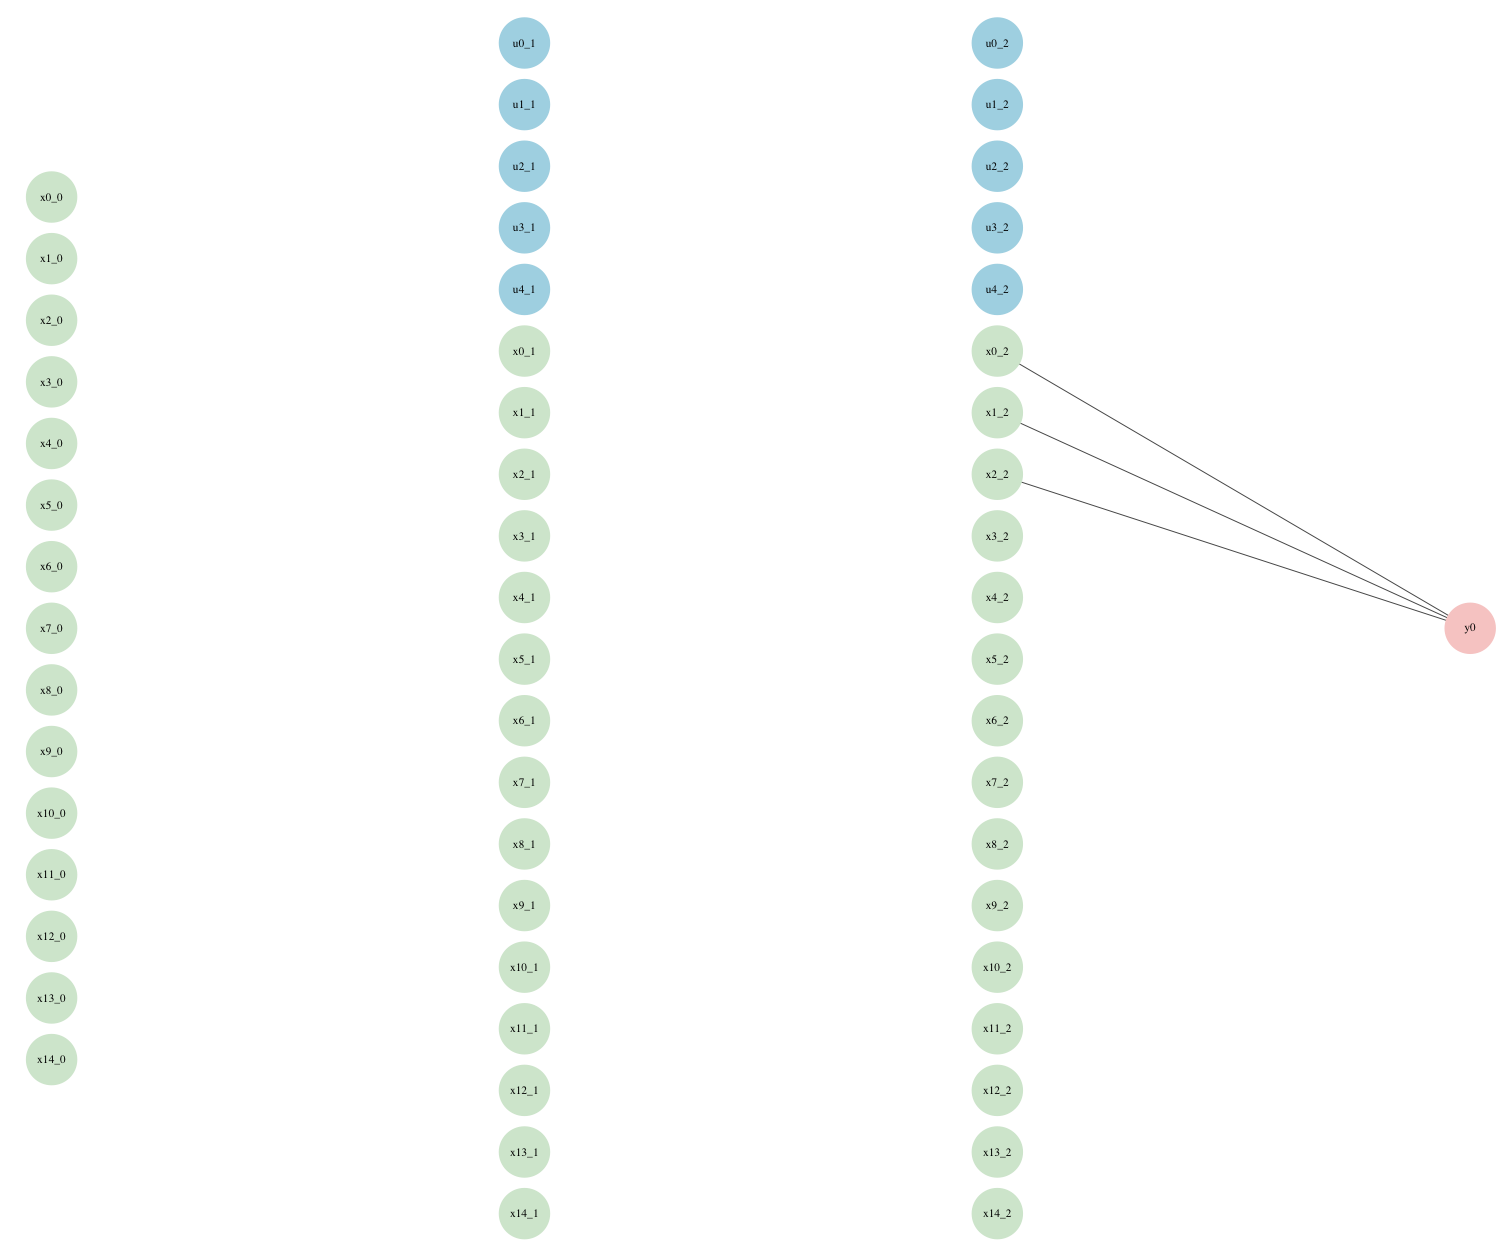
\includegraphics[width=0.9\textwidth]
    {figures/sim_linear_global.png}
    \caption{Global explanation for the network obtained in the simulation example with only linear effects.}
    \label{fig:global_linear_explanation}
\end{figure}
The plot can be seen in Figure \ref{fig:global_linear_explanation}. All connections are removed aside from the linear connections from the three data generating variables. To check if we recovered the true effects, we can obtain local explanations of predictions for some data samples of interest, using our version of \code{coef()} as follows:
\begin{example}
coef(model_linear, dataset = train_loader, inds = NULL,
     output_neuron = 1, num_data = 5, num_samples = 10)
\end{example}
The \code{dataset} argument refers to which dataset to use, it could be either a \code{torch::dataloader} object as in this case, or a user defined dataset. If the user wants to select specific samples from the dataset, then \code{inds} can be used to supply a vector of integers corresponding to the indices. If we have more than one output neuron (as in the case of multiclass classification), we get explanations for each output, \code{output\_neuron} controls which one to select. Further, \code{num\_data} refers to how many samples to select (randomly) from the given dataset, if no indices are provided. Lastly, \code{num\_samples} refers to how many samples to use for model averaging over the weights in active paths. We report the mean, and 95\% confidence/credible intervals for the explanations. If only one sample is used, the mean explanation and credible interval is given from model averaging over the weights. If multiple samples are selected, the overall mean explanation and confidence interval are derived from the individual mean explanations of each individual data sample.

For our example we obtain the following output:
\begin{example}
     lower      mean        upper
x0   0.5947226  0.6046016  0.6130178
x1  -0.4096843 -0.4018597 -0.3905376
x2   0.4884034  0.4964451  0.5038068
x3   0.0000000  0.0000000  0.0000000
...
x14  0.0000000  0.0000000   0.0000000
\end{example}
 The coefficients are very close to the true data generative ones, with only the first three variables included, as we wanted. If we only want to explain one specific sample, and also obtain the corresponding output, we can visualize this through the \code{plot()} function as follows:
\begin{example}
x <- train_loader$dataset$tensors[[1]] #grab the dataset
y <- train_loader$dataset$tensors[[2]] 
ind <- 42
data <- x[ind, ] #plot this specific data-point
output <- y[ind]
print(output$item()) #get the true y
[1] -0.8379451
plot(model_linear, type = "local", data = data)
\end{example}
The resulting plot can be seen in Figure \ref{fig:linear_explanation}.

\begin{figure}
    \centering
    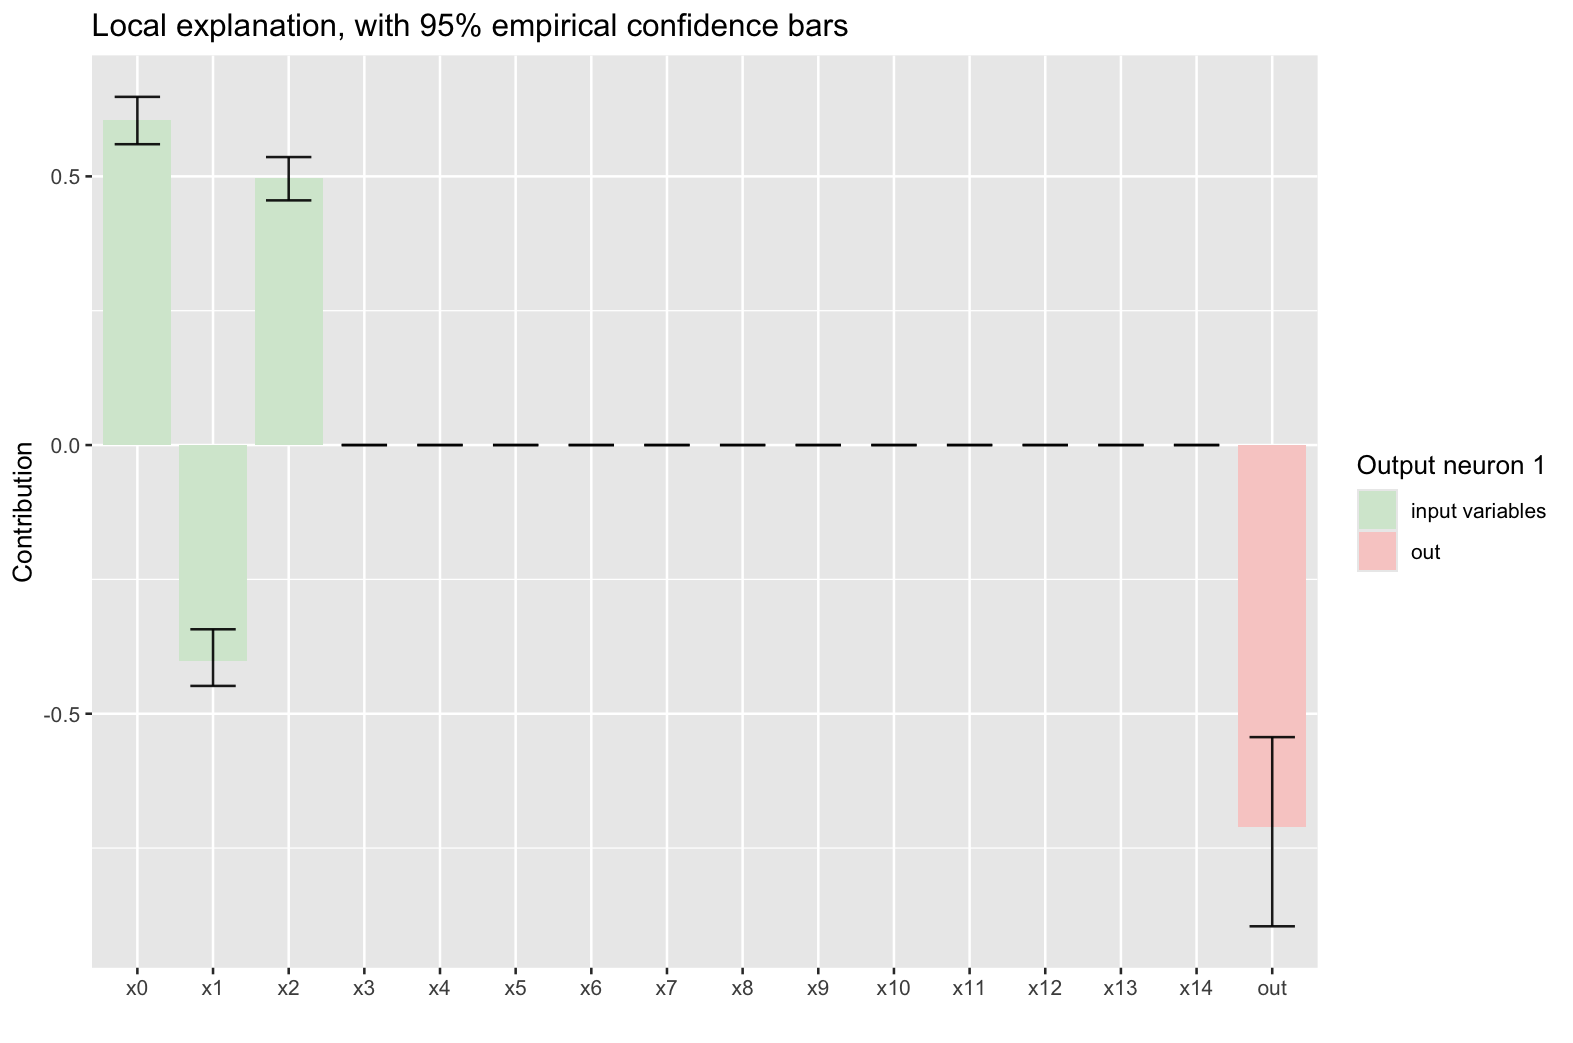
\includegraphics[width=1.0\textwidth]
    {figures/sim_linear_local.png}
    \caption{Local explanation with error bars for one sample in the simulation experiment with linear effects.}
    \label{fig:linear_explanation}
\end{figure}
For a quick overview of the model and its parameters, \code{print()} is useful: 
\begin{example}
    print(model_linear)

========================================
          LBBNN Model Summary           
========================================

Module Overview:
  - An `nn_module` containing 607 parameters.

---------------- Submodules ----------------
  - layers               : nn_module_list  # 545 parameters
  - layers.0             : lbbnn_linear    # 235 parameters
  - layers.1             : lbbnn_linear    # 310 parameters
  - act                  : nn_leaky_relu   # 0 parameters
  - out_layer            : lbbnn_linear    # 62 parameters
  - out                  : nn_identity     # 0 parameters
  - loss_fn              : nn_mse_loss     # 0 parameters

Model Configuration:
  - LBBNN with input-skip 
  - Optimized using variational inference without normalizing flows 

Priors:
  - Prior inclusion probabilities per layer:  0.5, 0.5, 0.5 
  - Prior std dev for weights per layer:     1, 1, 1 

=================================================================
\end{example}

\subsection{Tutorial 2: Simulation study with non-linear effects}
The data is generated in the following way:
\begin{align*}
    x_{ij}&\sim U(0,0.5)\\ \eta(\boldsymbol{x}_{i}) &= -3 +0.1\log(x_{i0})+3\cos(x_{i1}) +2x_{i2}x_{i3} +x_{i4} -x_{i5}^2 + \mathcal{N}(0,0.1),
\end{align*}
With $i = 1000$ and $j = 15$. In this case, we further transform the output into a binary variable: 
\begin{align*}
   {y_i} = 
    \begin{cases}
        0, \quad \eta(x_i) < \text{median}(\eta(x_i)) \\
        1, \quad \eta(x_i) \geq \text{median}(\eta(x_i)).
    \end{cases}
\end{align*}
Otherwise we use mostly the same hyperparameters as in the previous example, however since we now have a binary output, we specify:
\begin{example}
problem <- "binary classification"
\end{example}
In addition, we use normalizing flows, setting the argument \code{flow = TRUE} when initializing the model object. Training, otherwise, is done in exactly the same way as in the previous example. To check the results we again start with  \code{validate\_lbbnn}: 
\begin{example}
validate_lbbnn(LBBNN = model_nl, num_samples = 100, test_dl = test_loader_nl,
               device = device)
$accuracy_full_model
[1] 0.87

$accuracy_sparse
[1] 0.86

$density
[1] 0.1384615

$density_active_path
[1] 0.08717949
\end{example}
We get around 86\% accuracy with what appears to be a sparse network. To investigate the global structure of the network, we can use the \code{plot()} function again, specifying that we are interested in the global explanation:
\begin{example}
plot(model_nl, type = "global", vertex_size = 9,
     edge_width = 0.4, label_size = 0.4)
\end{example}

The results are displayed in Figure \ref{fig:simulation_ex}. From this, we see that all weights related to the irrelevant variables $x_6 -x_{14}$ have been pruned away, leaving us with a very sparse representation of effects for data-generating covariates. 
\begin{figure}[htb]
    \centering
    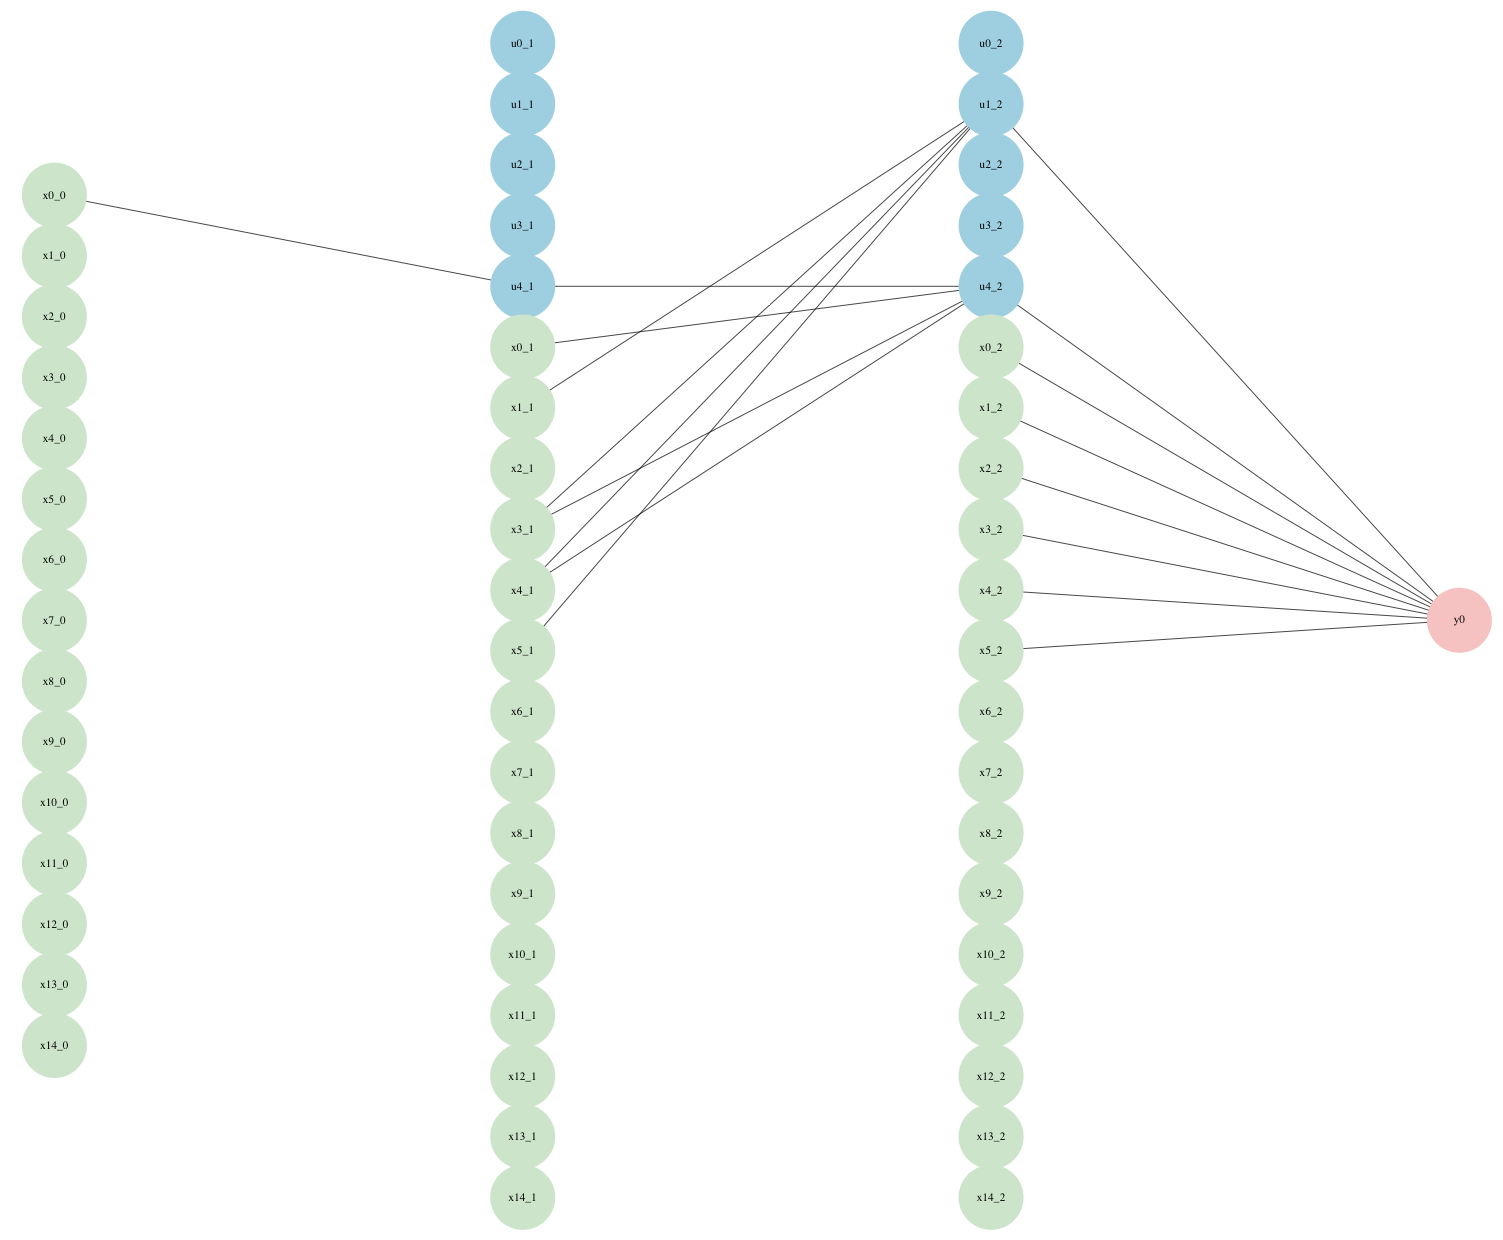
\includegraphics[width=.9\textwidth]
    {figures/sim_nonlinear_global.png}
    \caption{The structure of the network in the non-linear simulation example after removing weights that are not included in active paths.}
    \label{fig:simulation_ex}
\end{figure}

\subsection{Tutorial 3: Real data classification experiment}
For this experiment, we use the Gallstone dataset \citep{gallstone_1150} from the UCI machine learning repository. It consists of data from 319 individuals, where 161 were diagnosed with gallstone disease. It contains a mix of demographic, bioimpedance and laboratory covariates. The workflow is the same as in the previous example, so we skip the detailed description.  

For this problem, we use two hidden layers with three neurons in each, and train for 1000 epochs. We split the data 70/30 for training and validation, in line with the experiment described in \cite{gallstone_1150}, although we do not know the exact indices for the split, so the results may vary. In \cite{gallstone_1150}, the best result (85.42 $\%$) is obtained using gradient boosting. Our sparse input-skip model obtained an accuracy of $83.33\%$, using only roughly 5$\%$ of the total weights. 

The sparse structure is shown in Figure \ref{fig:gallstone_example}. We see that the entire first hidden layer has been pruned away, and only two of the three nodes in the last hidden layer are used. Additionally, many variables only have connections from the last layer.
\begin{figure}
    \centering
    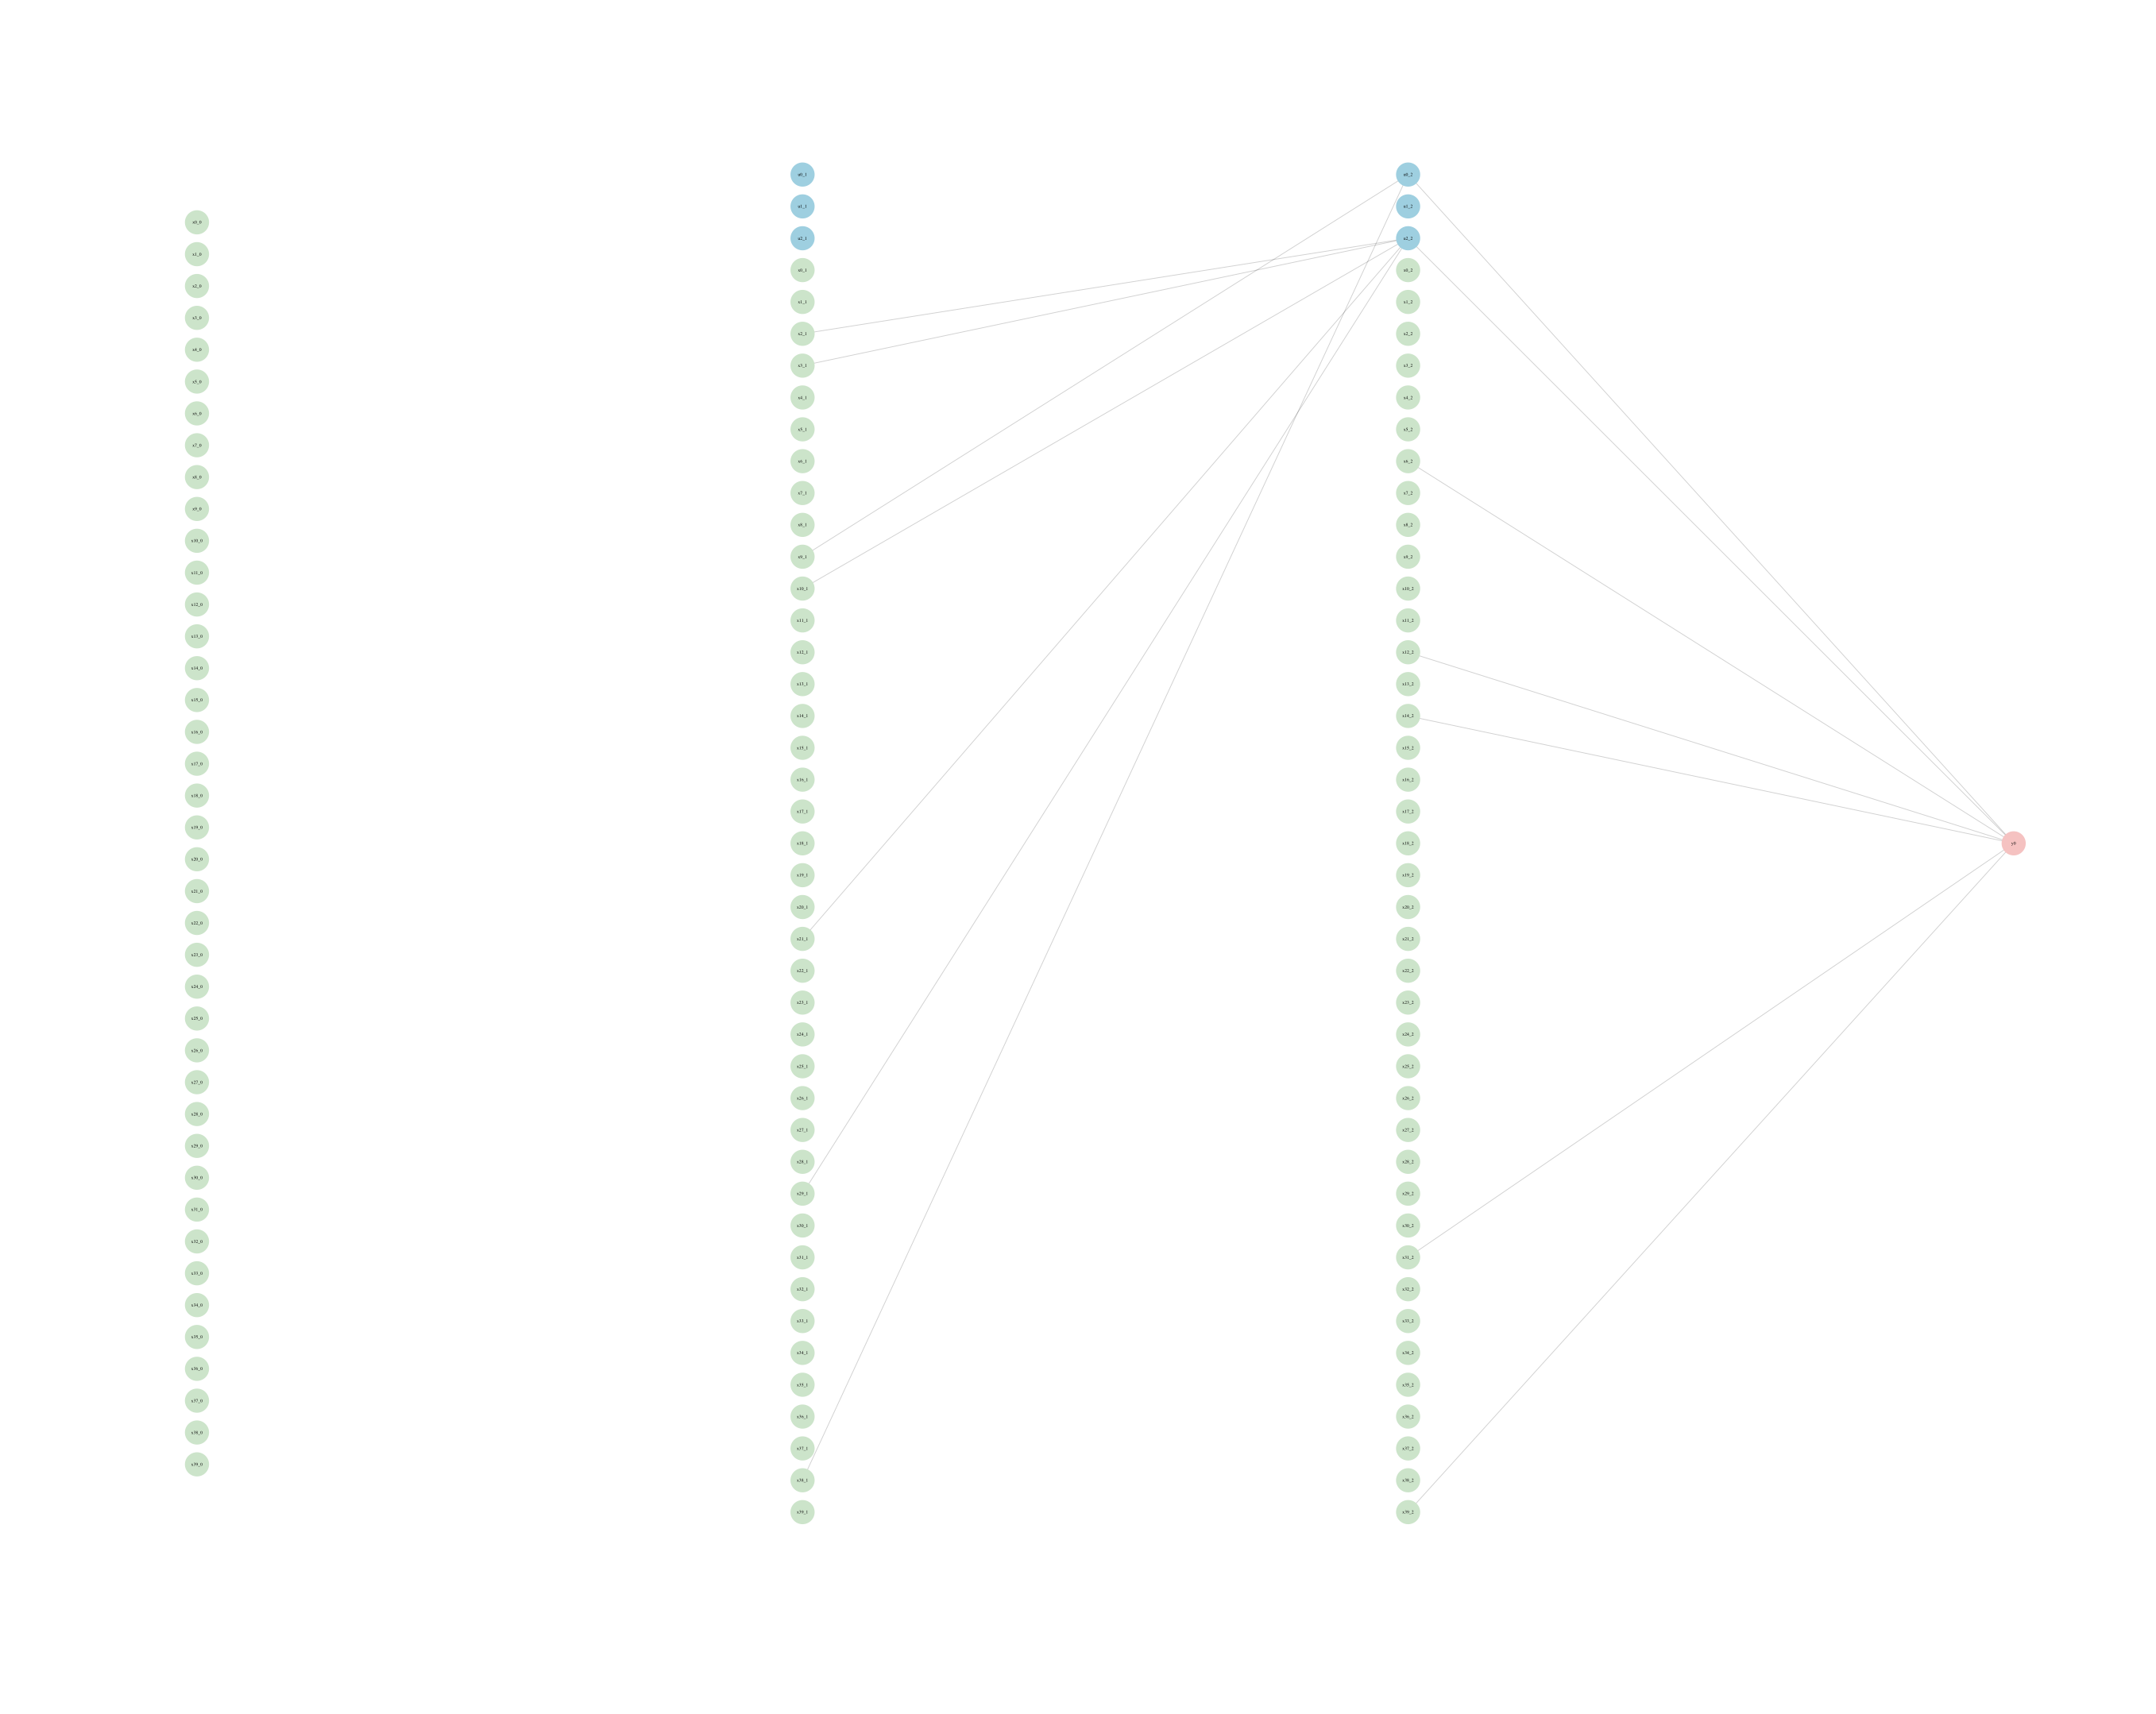
\includegraphics[width=0.8\textwidth]
    {figures/gallstone_global.png}
    \caption{The structure of the network in the gallstone data classification example after removing weights that are not included in active paths.}
    \label{fig:gallstone_example}
\end{figure}

Our package includes a few more standard R functions such as \code{predict()} and \code{residuals()} that we would like to demonstrate in this example. Below we show how to use the former:
\begin{example}
predictions_gs <- predict(model_gs, newdata = test_loader_gs,
                       draws = 100, mpm = TRUE)

\end{example}
Where \code{newdata} is the dataset to predict, \code{draws} refers to the number of posterior samples, and \code{mpm} refers to using the median probability model. The output of \code{predict} is the raw network outputs before sigmoid or softmax (or other link function) is applied. It is a three-dimensional tensor: 
\begin{example}
dim(predictions_gs)
[1] 100  96   1
\end{example}
where the axes correspond to draws, data points, and output units, respectively. For our case, the resulting tensor looks as:

\begin{example}
print(predictions_gs)
torch_tensor
(1,.,.) = 
-2.6755
0.2434
-3.2979
...
-1.3697
-0.3062
-1.5818
... [the output was truncated (use n=-1 to disable)]
[ CPUFloatType{100,96,1} ]
\end{example}

%\begin{figure}
 %   \centering
  %  \includegraphics[width=1.0\textwidth]
%    {figures/gallstone_data_local_expl.png}
 %   \caption{Local explanation with error bars for one sample taken from the gallstone dataset.}
 %   \label{fig:gallstone_explanation}
%\end{figure}

\subsection{Tutorial 4: Varying initializations on the raisin dataset}
Results (accuracy, final network structure) can be sensitive to some hyperparameters such as number of epochs, or the initializations of the probability of the inclusion parameters. 
% This is partially due to the nature of the dataset, which only consists of 319 samples. 
More generally, LBBNNs (with or without input-skip) can present optimization challenges, as the joint optimization over weights and inclusion parameters may lead to unstable training dynamics. The commonly used Adam optimizer, which we employ, was not designed for this type of problem. In future work, we aim to develop optimization strategies specifically tailored to LBBNNs.

This example will go into more detail on initialization strategies for the inclusion probabilities, and will present the user with different options. As mentioned previously, they are initialized as follows: 
\begin{align*}
    U &\sim\texttt{Uniform(a,b)} \\
    \alpha_{\texttt{init}}&=\texttt{sigmoid}(U).
\end{align*}
As an alternative to providing the values for \texttt{a} and \texttt{b}, we allow the user to also submit the keywords found in Table \ref{bernoulli_inits}. Figure \ref{fig:inits} provides a visualization of the initial distribution of the resulting Bernoulli probabilities, $\alpha_{\texttt{init}}$.
\begin{table}[htb]%[H]
\caption{Initialization ranges for the logits of the Bernoulli probabilities.}
\label{bernoulli_inits}
\begin{tabular}{@{}lrrrrrrr@{}}
\toprule
Keyword                                  & balanced   & dense  & polarized & polarized\_dense & polarized\_mild & polarized\_sparse & sparse \\ \midrule
a                                        & -1         & 1.5    & -10       & -5               & -3              & -10               & -2.5   \\
b                                        & 1          & 2.5    & 10        & 10               & 3               & 5                 & -1.5   \\ \midrule
a $\rightarrow \alpha_{\texttt{lower}}$  & 0.27       & 0.82   & $\sim$0   & 0.01             & 0.05            & $\sim$0           & 0.08   \\
b $\rightarrow \alpha_{\texttt{upper}}$  & 0.73       & 0.92   & $\sim$1   & $\sim$1          & 0.95            & 0.99              & 0.18   \\ \bottomrule
\end{tabular}
\end{table}

\begin{figure}[htb]%[H]
    \centering
    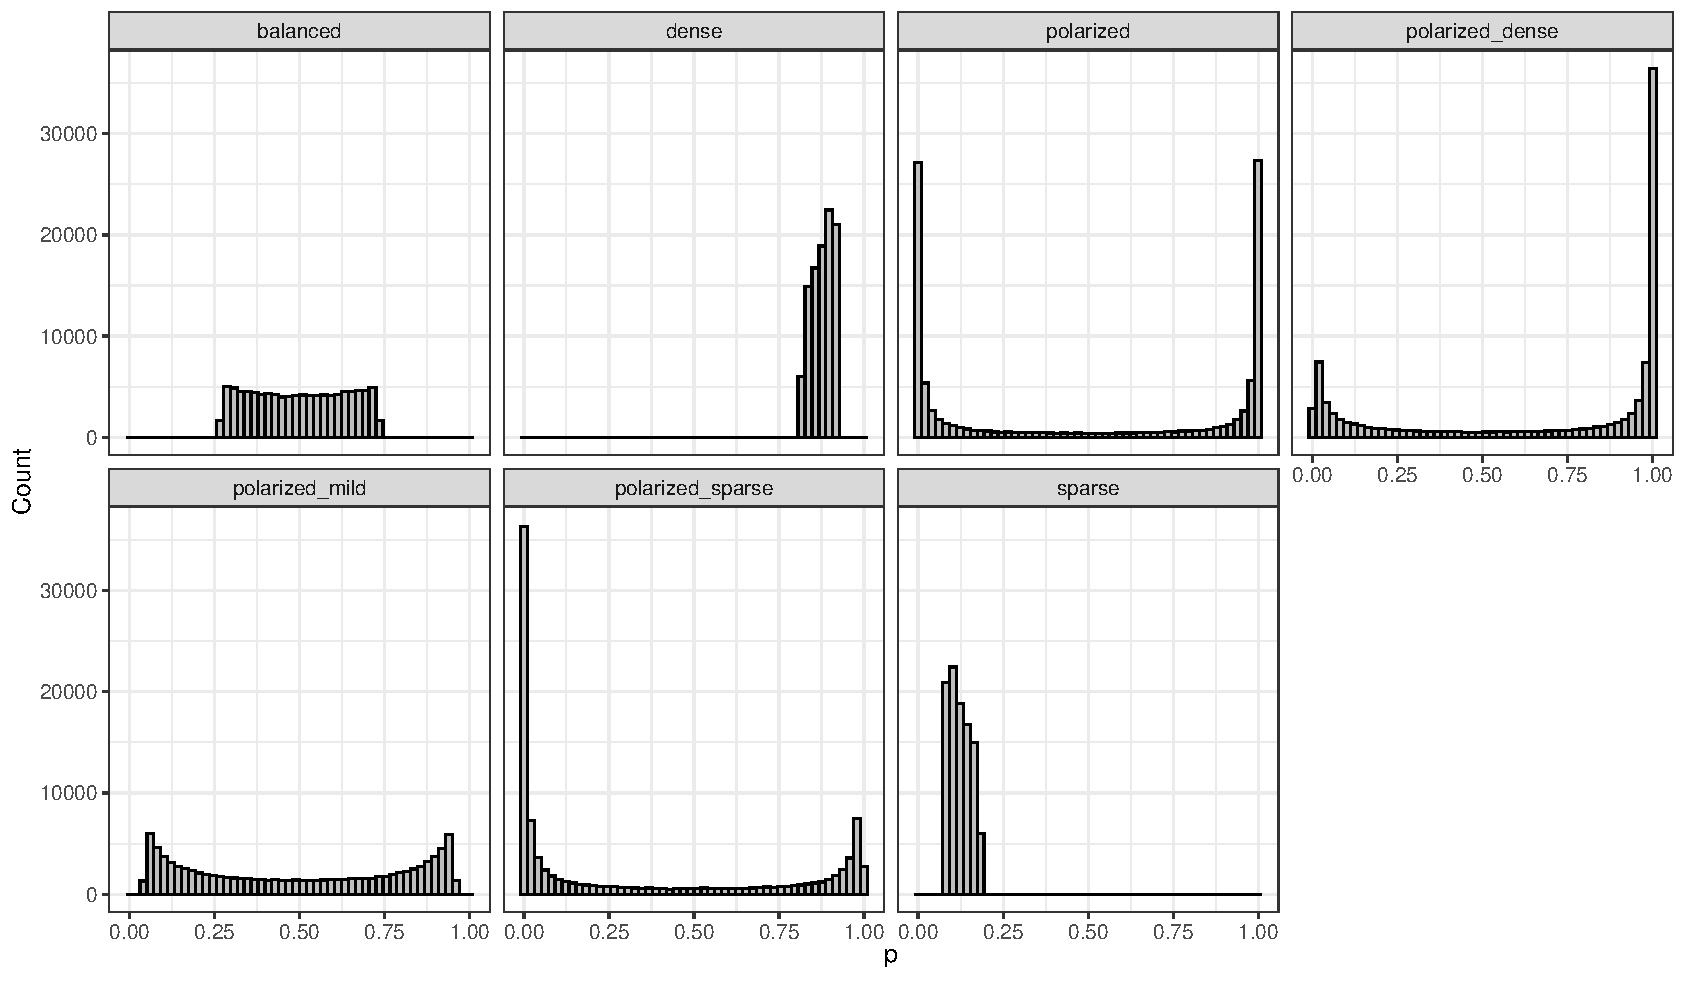
\includegraphics[width=1.0\linewidth]{figures/inits.pdf}
    \caption{Empirical distributions of initial inclusion probabilities for different initialization schemes.}
    \label{fig:inits}
\end{figure}

In the following experiment, we use the raisin dataset \citep{ccinar2020classification}, consisting of 900 samples, where the goal is to classify two types of raisins based on 7 morphological features. We use a network with 3 hidden layers, each consisting of 10 neurons. Of the 900 samples, 720 are used for training and 180 for validation. We compare results with different initialization, where the model is now defined as: 

\begin{example}
model_raisins <- lbbnn_net(problem_type = problem,sizes = sizes,
                           prior = inclusion_priors, 
                           inclusion_inits = 'balanced',input_skip = TRUE,
                           std = stds, flow = FALSE, device = device)
\end{example}
\begin{figure}[htb]%[H]
    \centering
    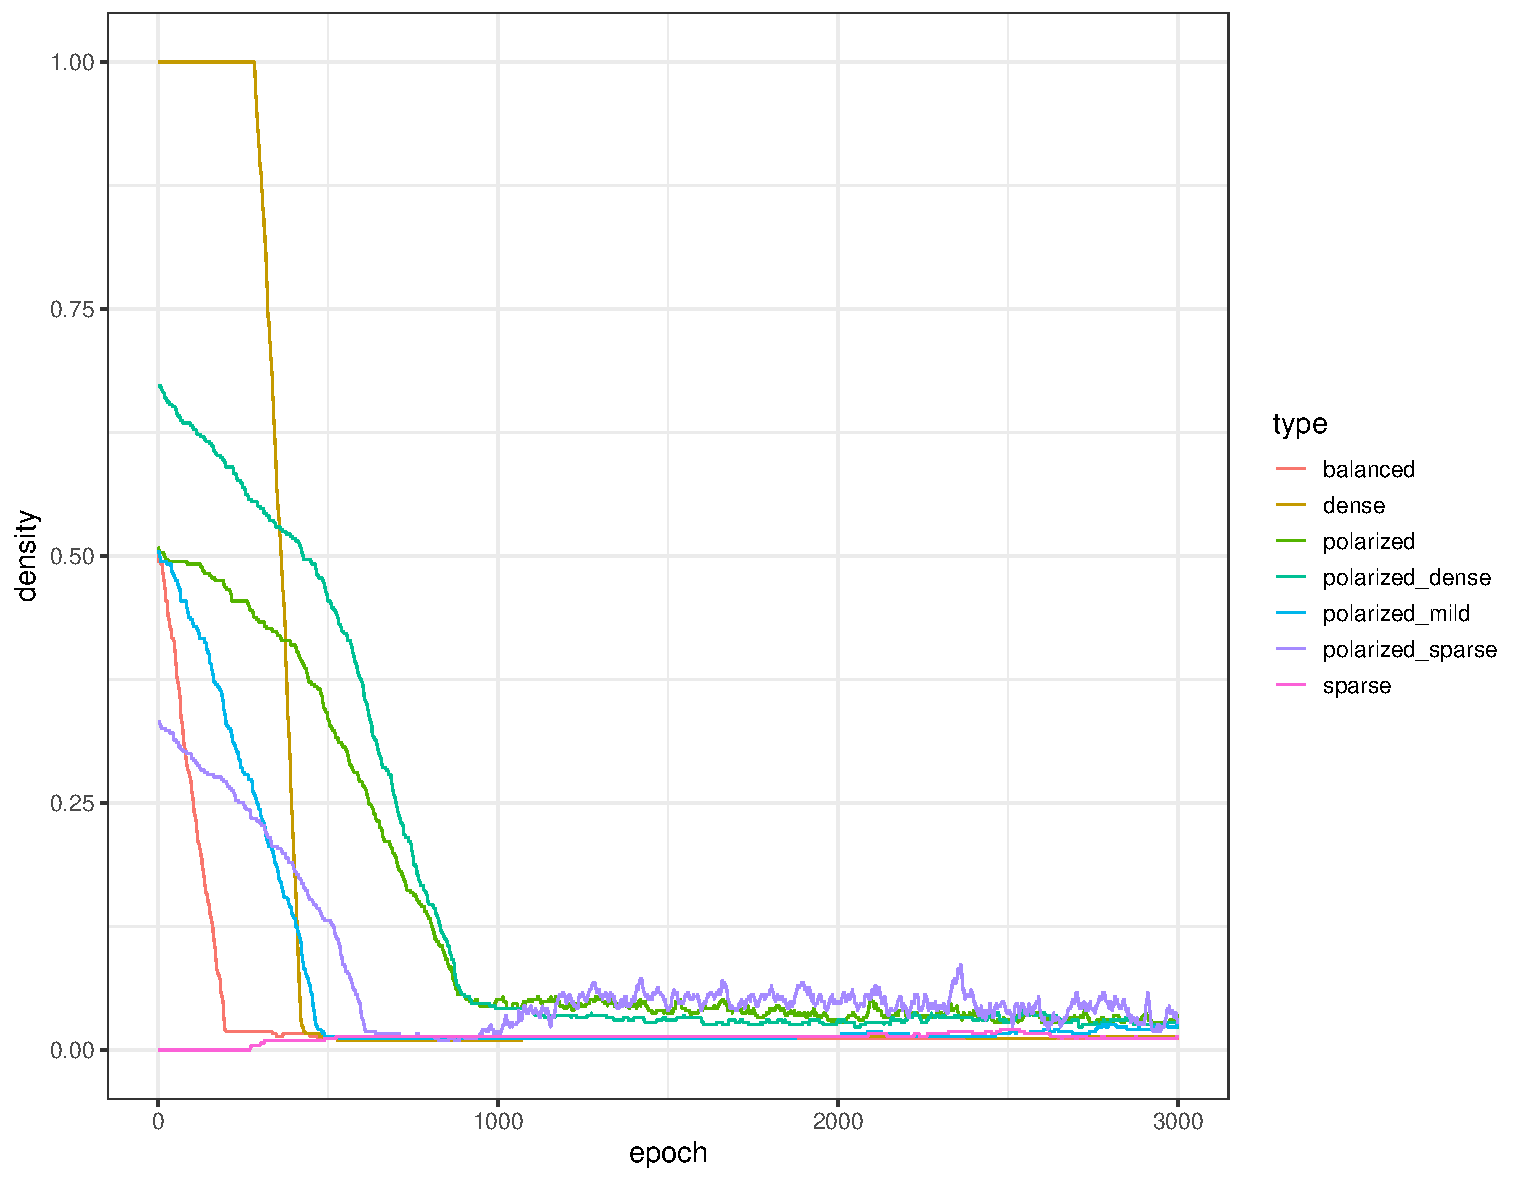
\includegraphics[width=1.0\linewidth]{figures/density.pdf}
    \caption{Density across epochs with different initializations.}
    \label{fig:density}
\end{figure}

Figure \ref{fig:density} displays the densities during training for the different initializations. In the dense case, the density is 1 for around 300 epochs, before it quickly approaches something close to 0. We see that the polarized options take longer to converge to low sparsities, but in the end, all initializations lead to very sparse networks after training for 3000 epochs. As a very low density may not be desirable in all situations, we include a tuning parameter for the minimum allowed density, such that training is terminated if this value is reached. It can be done using the \code{min\_density} keyword inside the \code{train\_lbbnn} function:
\begin{example}
results_raisins <- train_lbbnn(epochs = 3000,LBBNN = model_raisins, lr = 0.005,
                               train_dl = train_loader_raisin, device = device,
                               min_density = NULL)
\end{example}
For this example, we did not use a minimum density, but trained for 3000 epochs, to ensure convergence. The results on the validation data can be seen in Table \ref{raisin_results}. We see that the resulting networks are very sparse, using around $1-2\%$ of the weights. Despite this, accuracy is good and comparable to the results reported in the original paper \citep{ccinar2020classification}, 0.8633 accuracy using a frequentist neural network. In Figure \ref{fig:raisins_global} the global structures with the different initializations are shown.

\begin{table}
\caption{Performance and sparsity metrics on validation data on the raisins dataset.}
\label{raisin_results}
\centering
\begin{tabular}[t]{lrrrr}
\toprule
Initialization & accuracy & sparse accuracy & density & density active paths\\
\midrule
balanced & 0.8556 & 0.8556 & 0.0118 & 0.0118\\
dense & 0.8611 & 0.8667 & 0.0141 & 0.0141\\
polarized & 0.8667 & 0.8722 & 0.0351 & 0.0258\\
polarized\_dense & 0.8556 & 0.8556 & 0.0234 & 0.0211\\
polarized\_mild & 0.8611 & 0.8611 & 0.0258 & 0.0141\\
polarized\_sparse & 0.8556 & 0.8556 & 0.0281 & 0.0094\\
sparse & 0.8722 & 0.8611 & 0.0141 & 0.0094\\
\bottomrule
\end{tabular}
\end{table}

\begin{figure}[htbp]
\centering
\begin{subfigure}{0.24\textwidth}
    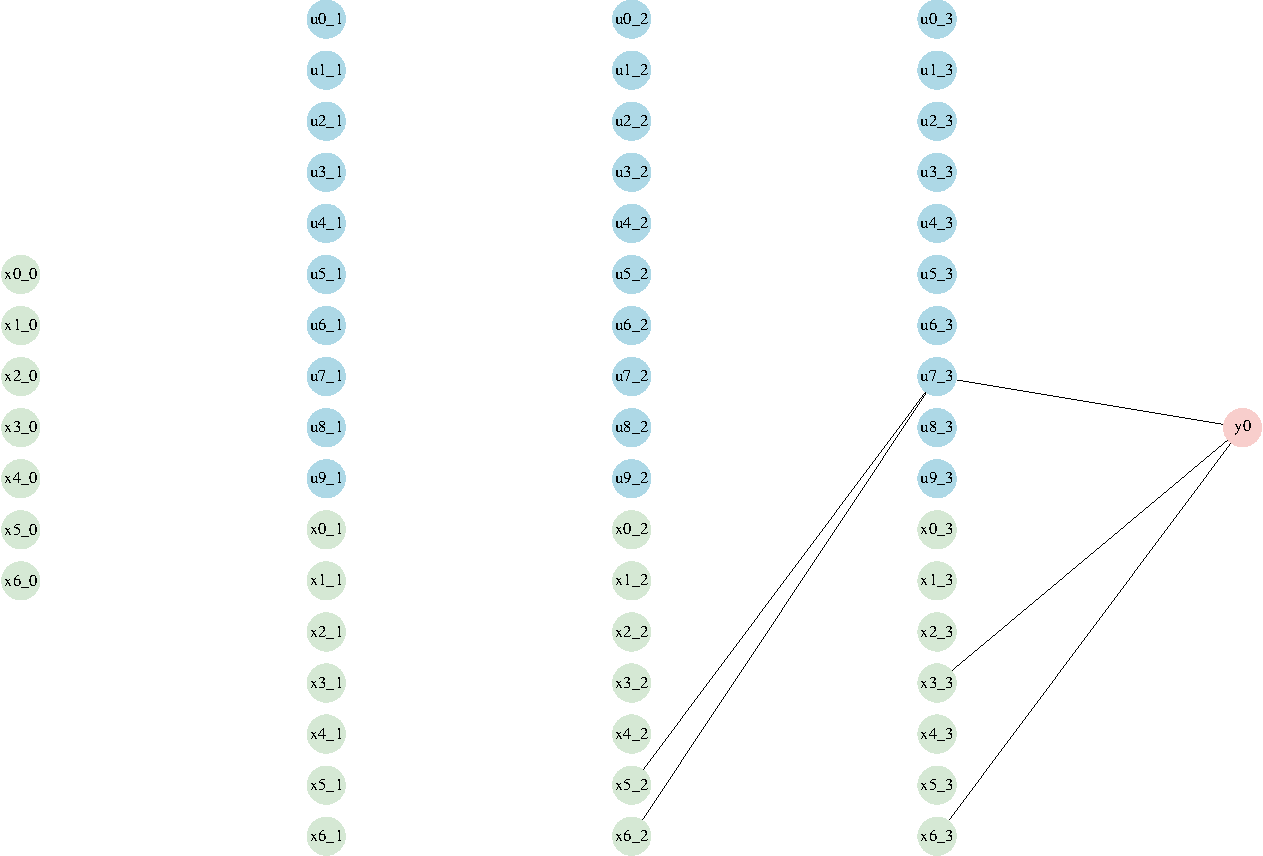
\includegraphics[width=\linewidth]{figures/raisins_balanced.pdf}
    \caption{balanced}
\end{subfigure}
\begin{subfigure}{0.24\textwidth}
    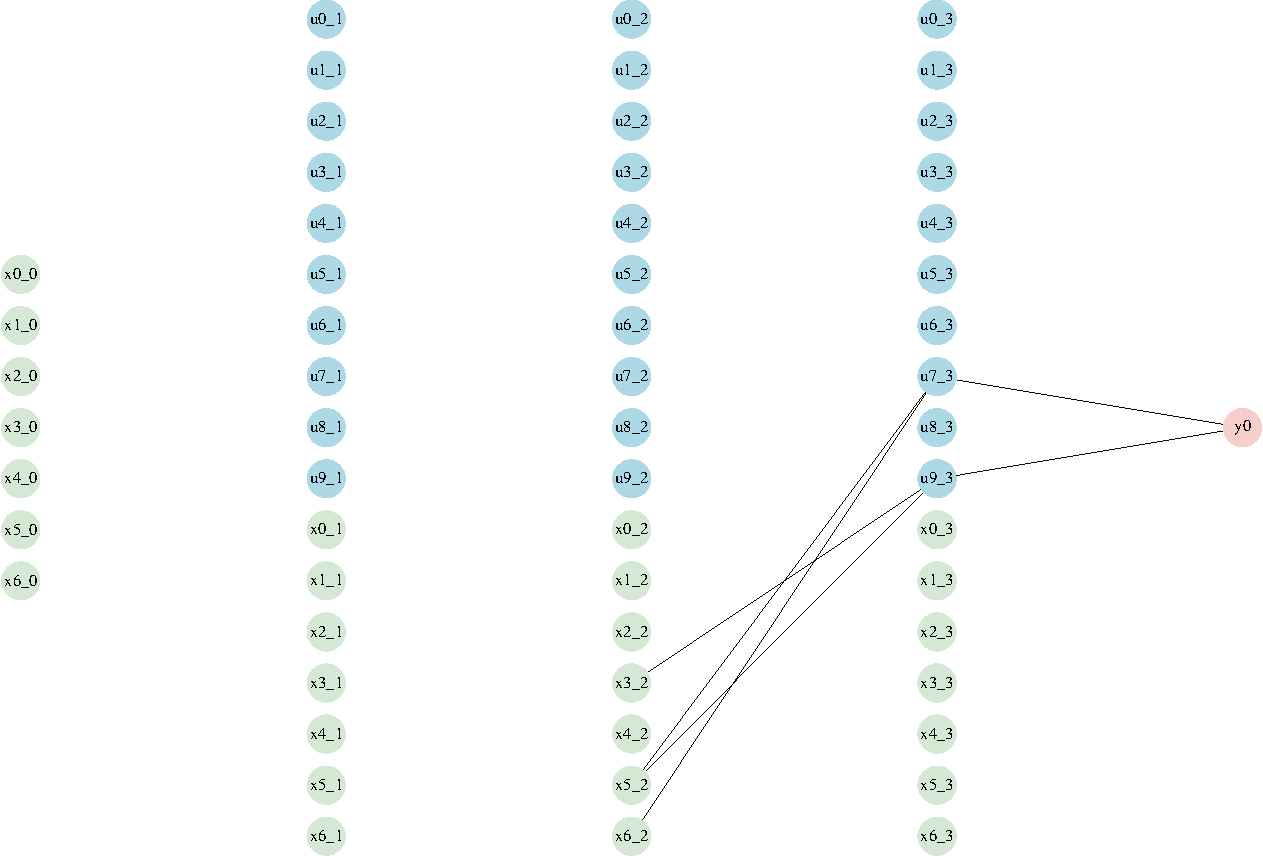
\includegraphics[width=\linewidth]{figures/raisins_dense.pdf}
    \caption{dense}
\end{subfigure}
\begin{subfigure}{0.24\textwidth}
    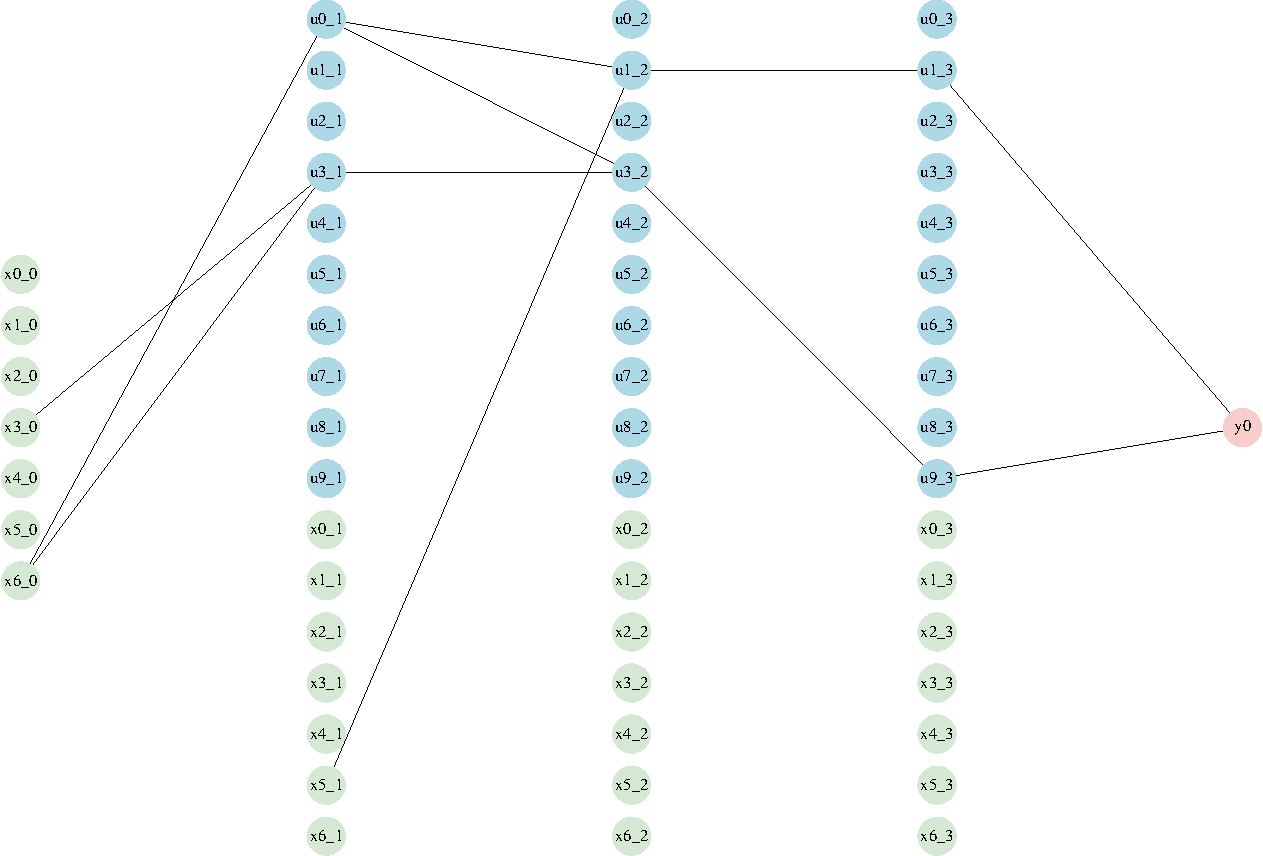
\includegraphics[width=\linewidth]{figures/raisins_polarized.pdf}
    \caption{polarized}
\end{subfigure}
\begin{subfigure}{0.24\textwidth}
    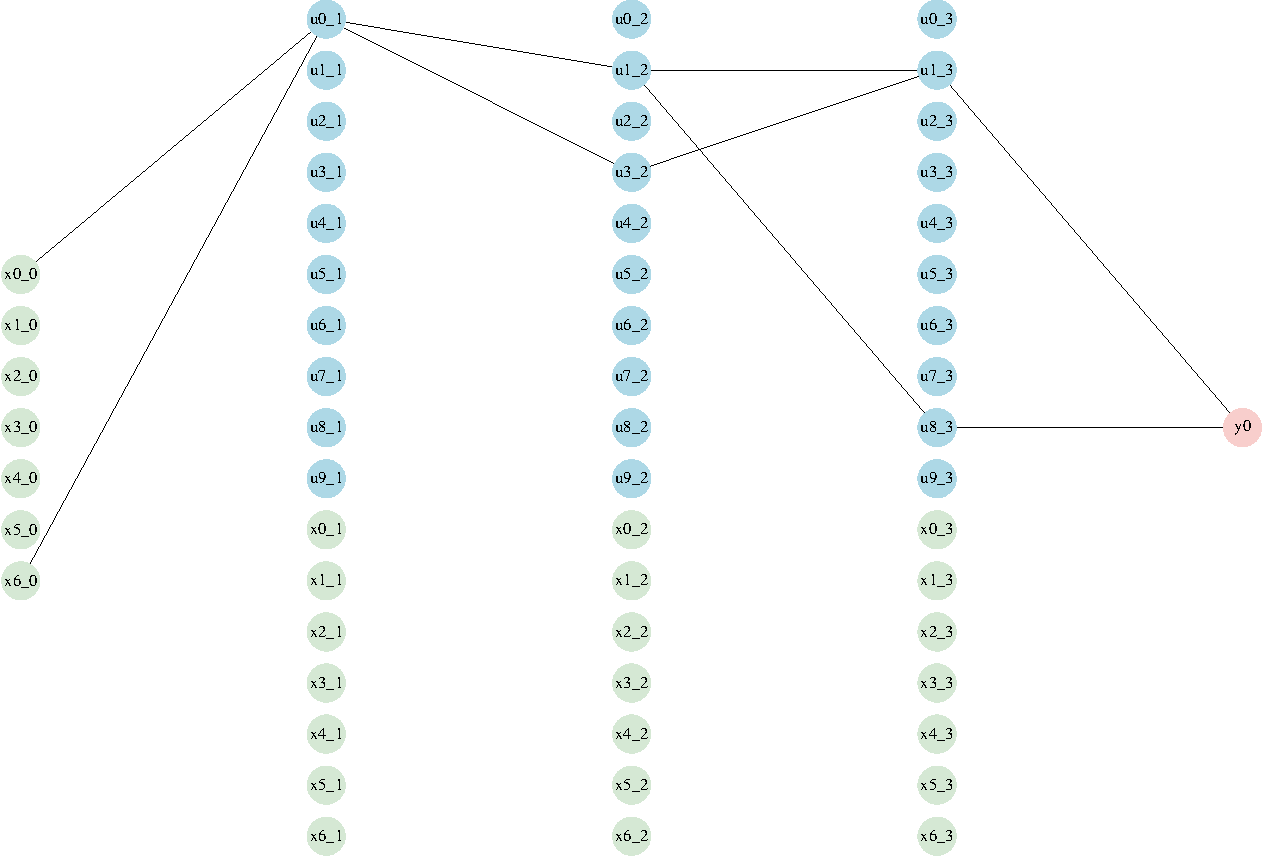
\includegraphics[width=\linewidth]{figures/raisins_polarized_dense.pdf}
    \caption{polarized\_dense}
\end{subfigure}

\vspace{0.2cm}

\begin{subfigure}{0.24\textwidth}
    \centering
    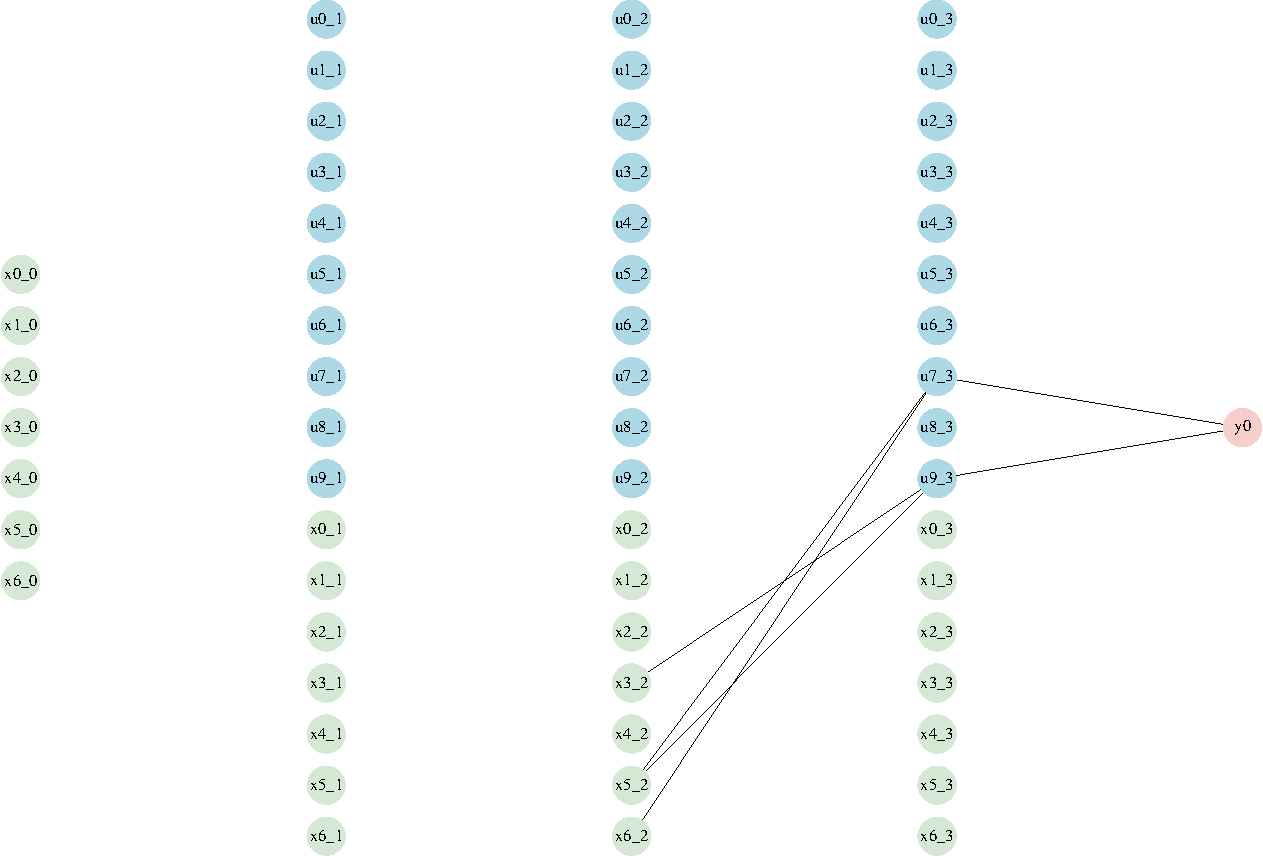
\includegraphics[width=\linewidth]{figures/raisins_polarized_mild.pdf}
    \caption{polarized\_mild}
\end{subfigure}
\begin{subfigure}{0.24\textwidth}
    \centering
    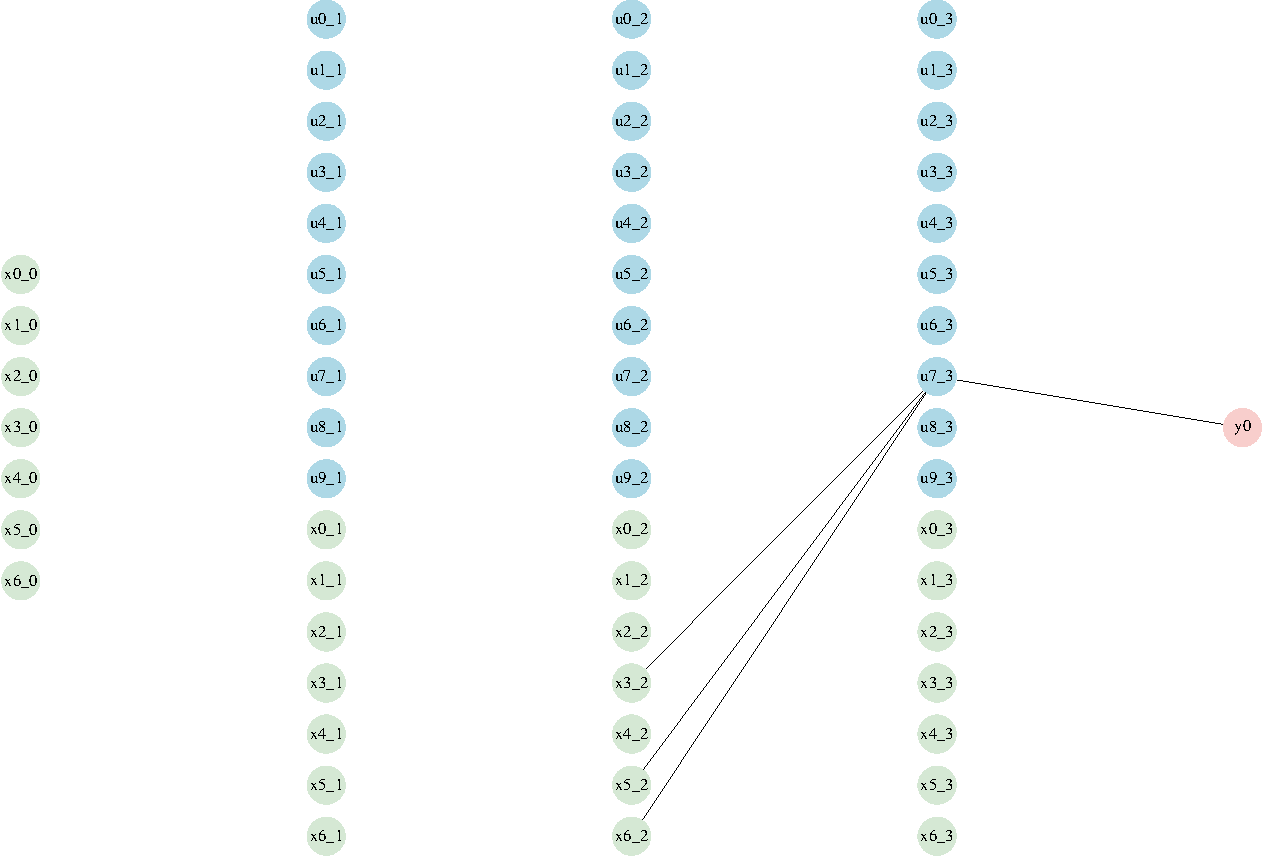
\includegraphics[width=\linewidth]{figures/raisins_polarized_sparse.pdf}
    \caption{polarized\_sparse}
\end{subfigure}
\begin{subfigure}{0.24\textwidth}
    \centering
    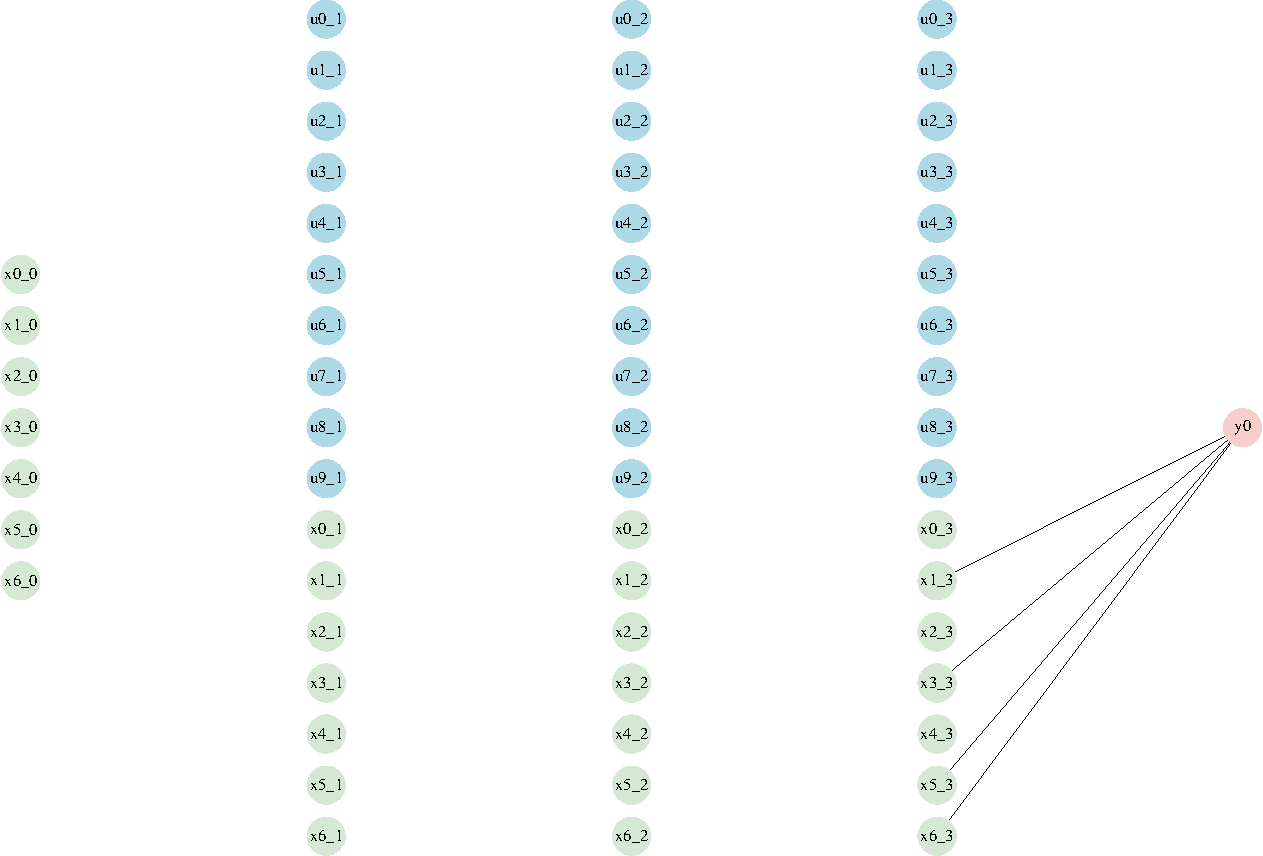
\includegraphics[width=\linewidth]{figures/raisins_sparse.pdf}
    \caption{sparse}
\end{subfigure}
\caption{Comparison of the global structure of the networks after training with different initializations on the raisin dataset.}\label{fig:raisins_global}
\end{figure}

\color{black}

\subsection{Tutorial 5: Extending the LBBNN to a convolutional architecture}
In this tutorial, we demonstrate an example on how to extend LBBNN. The specific extension is a Bayesian convolutional neural network (CNN), using \code{lbbnn\_linear} and \code{lbbnn\_conv2d} for feed-forward and convolutional LBBNN layers respectively. We have previously used \code{lbbnn\_linear} layers internally when defining \code{lbbnn\_net} objects, but here we will go into more details about how to explicitly define the layers needed in a CNN architecture. We do not use input-skip in this example, for simplicity.

We use the KMNIST dataset \citep{clanuwat2018deep}, consisting of 70,000 grayscale images (28x28 pixels) of handwritten Japanese Hiragana characters, with 10 different classes, providing a much larger and higher dimensional dataset than the previous examples. KMNIST is considered a more challenging alternative to the classical MNIST dataset, commonly used to benchmark novel machine learning methods. Some examples of what these images look like can be seen in Figure \ref{fig:kmnist_grid}.

\begin{figure}[htb]%[H]  
    \centering
    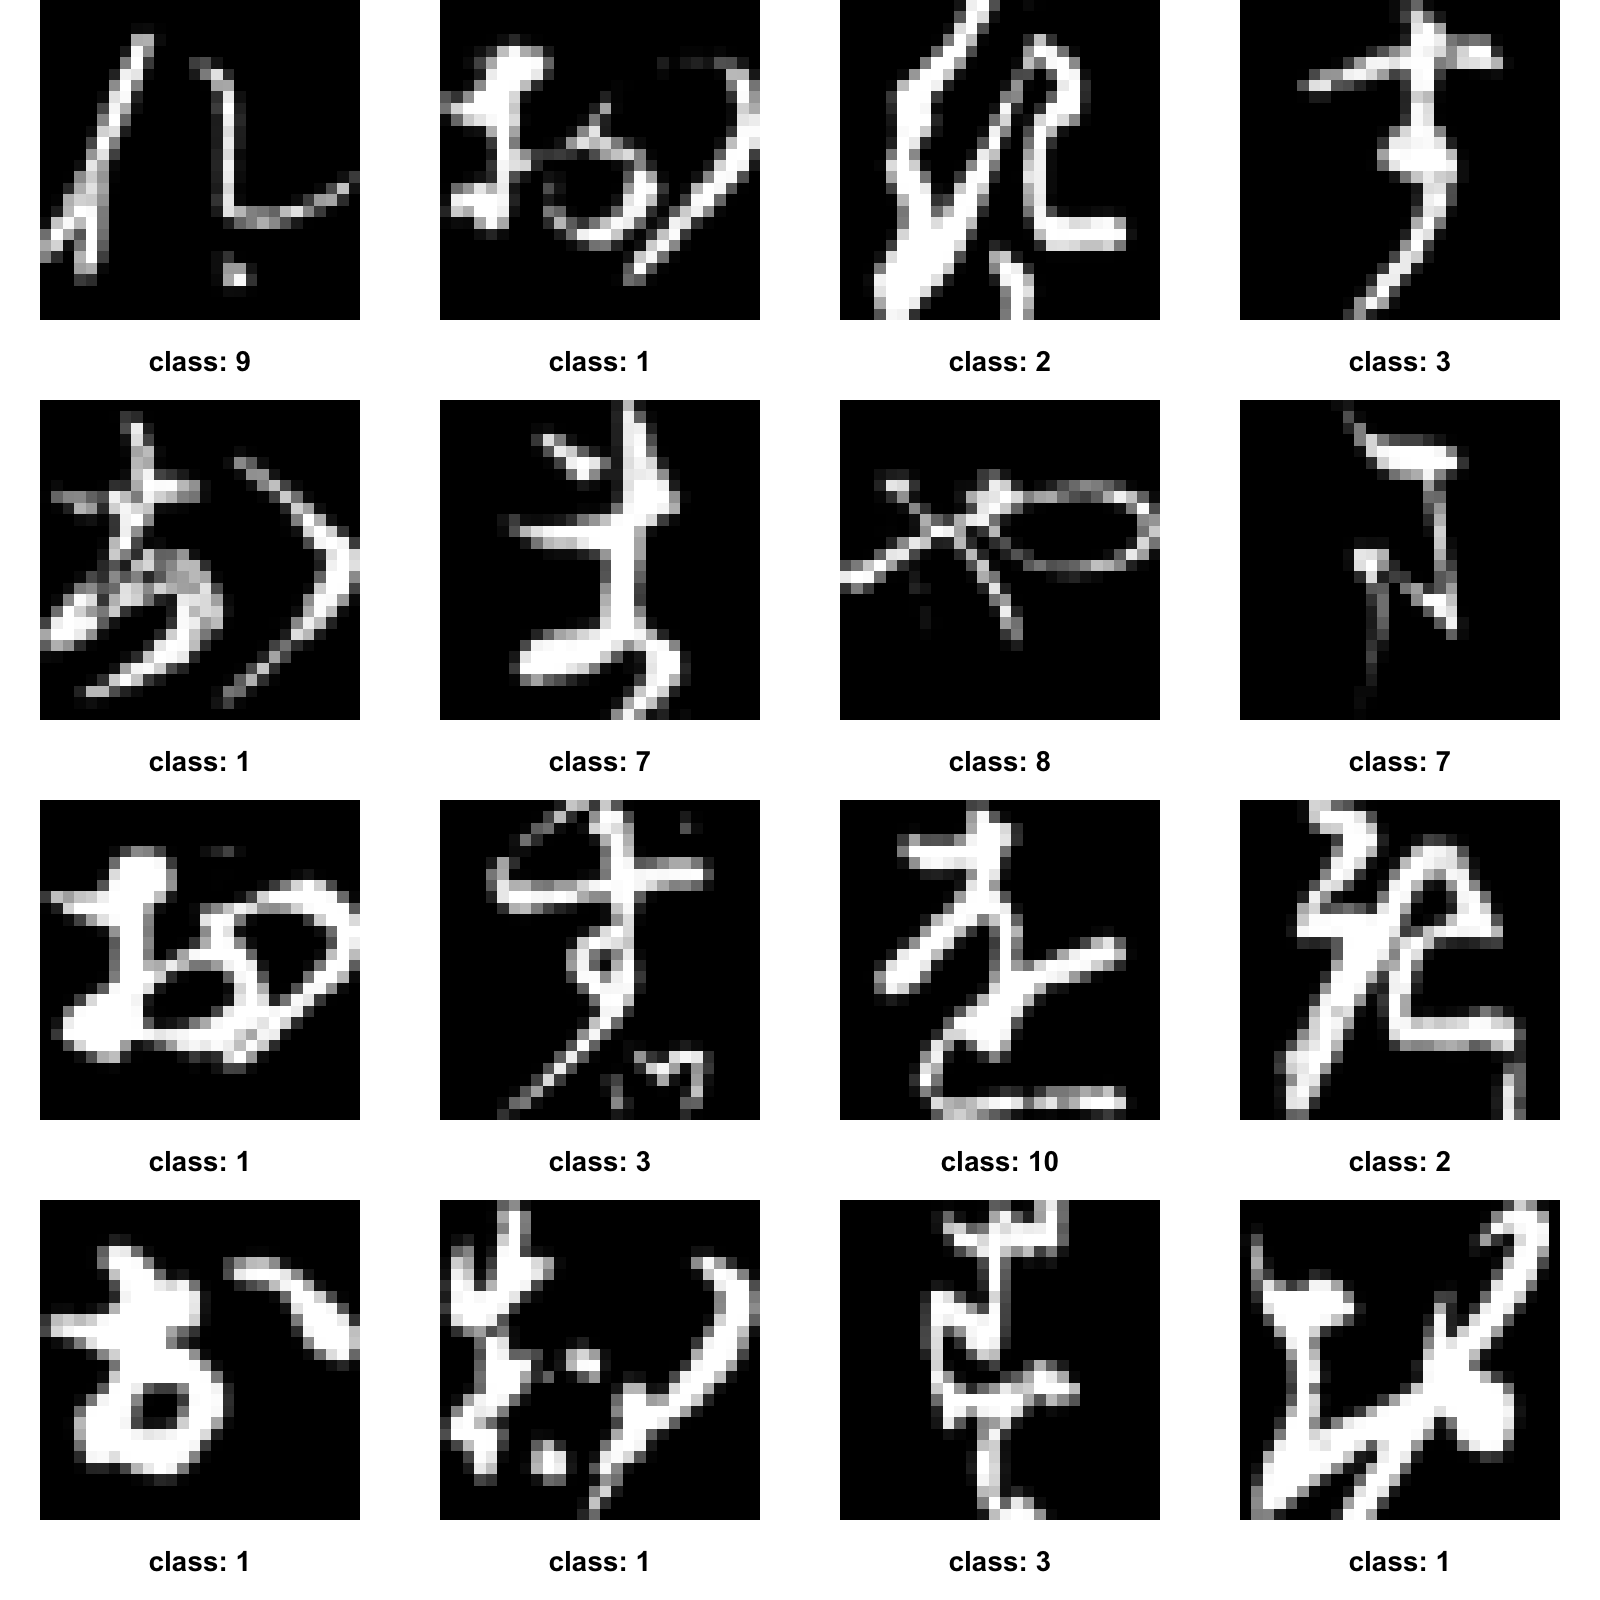
\includegraphics[width=0.7\textwidth]{figures/kmnist_grid_labeled.png}
    \caption{Random 4×4 grid of KMNIST images with class labels.}
    \label{fig:kmnist_grid}
\end{figure}

To begin, we download the dataset using the \code{torchvision} package, and create dataloaders, this time using \code{torch} directly:
\begin{example}
torch::torch_manual_seed(42)

dir <- "./dataset/kmnist"
train_ds <- torchvision::kmnist_dataset(
   dir,
   download = TRUE,
   transform = torchvision::transform_to_tensor)

test_ds <- torchvision::kmnist_dataset(
  dir,
  train = FALSE,
  transform = torchvision::transform_to_tensor)

# define dataloaders 
train_loader_kmnist <- torch::dataloader(train_ds, batch_size = 100, shuffle = TRUE)
test_loader_kmnist <- torch::dataloader(test_ds, batch_size = 100)
\end{example}
The dataset is split into 60,000 training samples and 10,000 test samples, loaded into the corresponding dataloaders. For the CNN architecture, we use two convolutional layers, and then two fully connected layers. The convolutional layers are defined as follows:
\begin{example}
device <- "cpu"
conv_layer_1 <- lbbnn_conv2d(in_channels = 1, out_channels = 32, kernel_size = 5,
                             prior_inclusion = 0.5, standard_prior = 1,
                             density_init = c(-10, 10), num_transforms = 2,
                             flow = FALSE, hidden_dims = c(200, 200),
                             device = device)
conv_layer_2 <- lbbnn_conv2d(in_channels = 32, out_channels = 64, kernel_size = 5,
                             prior_inclusion = 0.5, standard_prior = 1,
                             density_init = c(-10, 15), num_transforms = 2,
                             flow = FALSE, hidden_dims = c(200, 200),
                             device = device)
\end{example}
Here, we used \code{'cpu'} device for compatibility across platforms, however for this example to run faster, we recommend using \code{'gpu'} or \code{'mps'} devices upon availability \footnote{For this specific example we achieved 1.7x speedup on a NVIDIA RTX 6000 Ada Generation 48GB GPU versus an Intel® Xeon® E5-2680 v4 @ 2.40GHz (56 threads) CPU, and when increasing batch size to 512 we got 2.1x speedup.}. Further, \code{in\_channels} refers to the number of input channels to the layer, which is 1 for grayscale images such as KMNIST. \code{out\_channels} refers to the number of channels or feature maps produced by the convolutional layer. \code{kernel\_size} specifies the dimensions of the convolutional filter applied to the input. For example, a \code{kernel\_size} of 5 corresponds to a 5x5 filter. The rest of the arguments are the same as those used to define \code{lbbnn\_net} objects in previous examples. Further, we define the following fully-connected layers:
\begin{example}
linear_layer_1 <- lbbnn_linear(in_features = 1024, out_features = 300,
                         prior_inclusion = 0.5, standard_prior = 1,
                         density_init = c(-10, 10), num_transforms = 2,
                         flow = FALSE, hidden_dims = c(200, 200), device = device,
                         bias_inclusion_prob = FALSE, conv_net = TRUE)

linear_layer_2 <- lbbnn_linear(in_features = 300, out_features = 10,
                         prior_inclusion = 0.5, standard_prior = 1,
                         density_init = c(-5, 15),num_transforms = 2,
                         flow = FALSE, hidden_dims = c(200, 200), device = device,
                         bias_inclusion_prob = FALSE, conv_net = TRUE)
\end{example}
After pooling each convolutional layer and flattening the output of the final layer, we obtain 1,024 input features to the first layer, where \code{out\_features} refers to the number of hidden neurons in that layer. For the final layer, we have $10$ \code{out\_features}, as there are 10 possible classes. The argument \code{conv\_net} is used to skip the computation of active paths. The model class is defined as follows:
\begin{example}
LBBNN_ConvNet <- torch::nn_module(
  "LBBNN_ConvNet",

  initialize = function(conv1, conv2, fc1 ,fc2 ,device = device) {
    self$problem_type <- "multiclass classification"
    self$input_skip <- FALSE
    self$conv1 <- conv1
    self$conv2 <- conv2
    self$fc1 <- fc1
    self$fc2 <- fc2

    self$pool <- torch::nn_max_pool2d(2)
    self$act <- torch::nn_leaky_relu()
    self$out <- torch::nn_log_softmax(dim = 2)
    self$pout <- torch::nn_softmax(dim = 2)
    self$loss_fn <- torch::nn_nll_loss(reduction = "sum")
  },

  forward = function(x, MPM = FALSE, predict = FALSE) {
    x = self$act(self$conv1(x, MPM))
    x = self$pool(x)
    x = self$act(self$conv2(x, MPM))
    x = self$pool(x)
    x = torch::torch_flatten(x,start_dim = 2)
    x = self$act(self$fc1(x, MPM))
    if(!predict)
      x = self$out(self$fc2(x ,MPM))
    else
      x = self$pout(self$fc2(x ,MPM))
  },
  kl_div = function(){
    kl <- self$conv1$kl_div() + self$conv2$kl_div() +
      self$fc1$kl_div() + self$fc2$kl_div()
    return(kl)
  },
  density = function(){
    alphas <- NULL
    l1 <- self$conv1$lambda_l$clone()$detach()
    l2 <- self$conv1$lambda_l$clone()$detach()
    l3 <- self$fc1$lambda_l$clone()$detach()
    l4 <- self$fc2$lambda_l$clone()$detach()
    alphas <- c(as.numeric(torch::torch_sigmoid(l1)),
                as.numeric(torch::torch_sigmoid(l2)),
                as.numeric(torch::torch_sigmoid(l3)), 
                as.numeric(torch::torch_sigmoid(l4)))
    return(mean(alphas > 0.5))
  },
  compute_paths = function(){
    NULL
  },
  density_active_path = function(){
    NA
  }
)
\end{example}
The \code{initialize} method runs automatically each time an instance of \code{LBBNN\_ConvNet} is created, setting up the network layers and additional parameters. As well as the layers mentioned, we also define the pooling layer, output layer, activation function and loss function here. The method \code{forward} applies two convolutional layers, each followed by a LeakyReLU activation function and max-pooling. The resulting feature maps are flattened and passed through a fully connected layer with LeakyReLU, and then through a final output layer. The argument \code{MPM} refers to the median probability model. When \code{TRUE}, only weights with a corresponding inclusion probability greater than 0.5 are used. \code{predict} refers to whether the forward pass is used in the prediction mode, returning class probabilities. Further, \code{kl\_div} is used to compute the KL-divergence of the network, which is the sum of the individual KL-divergences between the prior and posterior (variational) distribution of the weights and inclusion parameters for each independent layer. This is added to the loss function of the network. To compute the density (proportion of weights in the network with inclusion probability larger than 0.5) we use the \code{density} method. Lastly, \code{compute\_paths} and \code{density\_active\_path} need to be defined (but not do anything) so that the same training and validation functions as in previous examples can be used. We can now define an instance of the model and move it to the device:
\begin{example}
model_kmnist <- LBBNN_ConvNet(conv_layer_1, conv_layer_2, linear_layer_1,
                       linear_layer_2, device)
model_kmnist$to(device = device)
\end{example}
We now use \code{train\_lbbnn}, training for $20$ epochs with a learning rate of $0.001$:
\begin{example}
train_lbbnn(epochs = 20, LBBNN = model_kmnist, lr = 0.001, train_dl = train_loader_kmnist,
            device = device)
\end{example}
During training, the loss, accuracy and density can be monitored just as in the standard LBBNN:
\begin{example}
Epoch 1, training: loss = 2861.02612, acc = 0.84528, density = 0.47281
Epoch 2, training: loss = 2516.05835, acc = 0.95975, density = 0.44291
Epoch 3, training: loss = 2209.72510, acc = 0.97410, density = 0.40780
...
Epoch 20, training: loss = 233.06529, acc = 0.95875, density = 0.03716
\end{example}
Finally, we validate the network on the unseen test data, with 10 samples for model averaging:
\begin{example}
validate_lbbnn(model_kmnist, num_samples = 10, test_dl = test_loader_kmnist, device = device)
\end{example}
Giving the following output:
\begin{example}
$accuracy_full_model
[1] 0.9355

$accuracy_sparse
[1] 0.9259

$density
[1] 0.03715523

$density_active_path
[1] NA
\end{example}
The accuracy is lower than during training, as one can expect. It could be improved by training for longer, or using normalizing flows as shown in \cite{skaaret-lund2024sparsifying}, but the purpose here is not to obtain the best possible results, but rather demonstrate how a simple convolutional LBBNN can be created. We note that convolutional LBBNNs can also be very sparse without sacrificing too much predictive power in this case. Active paths are not defined for convolutional architectures, hence density within them is not available for this example.

As we now are working with a different object than the standard \code{lbbnn\_net} object used earlier, our versions of generic R functions such as \code{summary()} and \code{coef()} will not work. We can still use \code{print()}, as this will use the \code{torch} version, and \code{LBBNN\_ConvNet} is a \code{torch::nn\_module} object. Below is the output:
\begin{example}
print(model_kmnist)
An `nn_module` containing 1,087,412 parameters.
--Modules --------------------------------
• conv1: <lbbnn_conv2d> #2,464 parameters
• conv2: <lbbnn_conv2d> #153,728 parameters
• fc1: <lbbnn_linear> #922,200 parameters
• fc2: <lbbnn_linear> #9,020 parameters
• pool: <nn_max_pool2d> #0 parameters
• act: <nn_leaky_relu> #0 parameters
• out: <nn_log_softmax> #0 parameters
• loss_fn: <nn_nll_loss> #0 parameters
\end{example}

The prediction function is not per default available for a convolutional network class, so we have to make predictions manually (or wrap it in a separate function). Below we show how to perform predictions manually:

\begin{example}
draws <- 20 # how many samples from posterior to use
out_dim <- 10 # dimensionality of the output
mpm <- TRUE # if to use the MPM
model_kmnist$eval() # to avoid gradient computations
predictions_kmnist <- NULL
torch::with_no_grad({ 
  coro::loop(for (b in test_loader_kmnist)# go through all data
  { 
    outputs <- torch::torch_zeros(draws,dim(b[[1]])[1],out_dim)$to(device=device)
    for(i in 1:draws)# go through all draws 
    {
      data <- b[[1]]$to(device = device)
      outputs[i]<- model_kmnist(data, MPM = mpm, predict = TRUE)
    }
    predictions_kmnist <- torch::torch_cat(c(predictions_kmnist, outputs), dim = 2) #combine all

  })  
})
\end{example}

Here we used 20 draws from the posterior per sample and we have 10 classes in the response. So, the dimension of the responses is 
\begin{example}
dim(predictions_kmnist)
[1]    20 10000    10
\end{example}
And we can take a look into the first 5 draws of the 255th\footnote{indexes are shuffled in torch data\_loaders, so results might differ on a different seed.} predicted image posteriors:
\begin{example}
idx1 <- min(255, dim(predictions_kmnist)[2])
print(torch::torch_round(predictions_kmnist[1:5, idx1, ], 4))

torch_tensor
 0.0096  0.0183  0.6126  0.0018  0.0215  0.0228  0.0546  0.2543  0.0028  0.0016
 0.0006  0.0002  0.9166  0.0020  0.0218  0.0180  0.0367  0.0020  0.0017  0.0002
 0.0018  0.0108  0.2626  0.0058  0.2404  0.3693  0.0863  0.0215  0.0003  0.0014
 0.0056  0.0463  0.1627  0.0050  0.0088  0.2112  0.2470  0.3102  0.0029  0.0003
 0.0001  0.0003  0.6468  0.0008  0.0056  0.3341  0.0116  0.0003  0.0004  0.0000
[ CPUFloatType{5,10} ]
\end{example}

In this specific case we see some uncertainty between different classes. If we look at the first 5 draws of the 258th predicted image posteriors, we see significant confidence in class 5:

\begin{example}
idx2 <- min(258, dim(predictions_kmnist)[2])
print(torch::torch_round(predictions_kmnist[1:5, idx2, ], 4))

torch_tensor
 0.0001  0.0001  0.0000  0.0000  0.9993  0.0000  0.0000  0.0003  0.0000  0.0001
 0.0017  0.0000  0.0001  0.0000  0.9947  0.0001  0.0003  0.0007  0.0002  0.0022
 0.0041  0.0035  0.0001  0.0005  0.7902  0.0021  0.0004  0.0136  0.0000  0.1854
 0.0001  0.0000  0.0000  0.0000  0.9987  0.0000  0.0010  0.0002  0.0000  0.0000
 0.0010  0.0005  0.0000  0.0001  0.9948  0.0001  0.0000  0.0024  0.0009  0.0002
[ CPUFloatType{5,10} ]
\end{example}

\section{Summary}
We have created a package that implements LBBNNs in R. It offers the possibility to use normalizing flows for a more flexible variational posterior distribution than the mean-field Gaussian. In addition, input-skip allows for a more flexible architecture where the concept of active paths can lead to very sparse representation, and thus obtaining global interpretability. While local explanations are further available and proven to be exact for piecewise linear activations. Our package is the first R package implementing LBBNNs using \code{torch}, facilitating GPU acceleration using the \code{LibTorch} backend. 

In our examples, we demonstrate how to use our package, both on toy data and real-world datasets. On the latter, our LBBNN model with input-skip obtains high accuracy with sparse networks, while also providing local explanations with uncertainty, easily accessible either through \code{coef()} (with the possibility of aggregating multiple samples) or for visualization of a single sample through \code{plot()}. Additional information about the model can be obtained through \code{summary()}, showing how many paths included each input variable from each layer, in addition to the average inclusion probability for each layer, and overall. The structure of the model and the number of total parameters can be seen through \code{print()}. We further provided an example on how to extend the package to work with convolutional architectures with image classification applications, demonstrating that our package can also handle high dimensional data. Further, the fundamental building blocks used in that example could also be used to create much deeper architectures, such as residual networks like ResNet-18, however, this would come at the cost of significantly more parameters compared to the roughly 1 million in our example.

Future work will focus on extending the LBBNN package to support deeper and more complex architectures like residual networks or transformers, explore alternative transformations for the normalizing flows, and, most importantly, develop novel LBBNN specific optimizers that can better handle model selection and the input-skip architecture in high-dimensional parameter settings.

\bibliography{LBBNN_article}

\address{Lars Skaaret-Lund\\
  KBM, Bioinformatics and applied statistics (BIAS),
Norwegian University of Life Sciences\\
  Elizabeth Stephansens v. 15, 1433 Ås\\
  Norway
  \\
  \email{lars.skaaret-lund@nmbu.no}}

\address{Eirik Høyheim\\
  KBM, Bioinformatics and applied statistics (BIAS),
Norwegian University of Life Sciences\\
  Elizabeth Stephansens v. 15, 1433 Ås\\
  Norway\\
  \email{eirik.hoyheim@ffi.no}}

\address{Aliaksandr Hubin\\
   KBM, Bioinformatics and applied statistics (BIAS),
Norwegian University of Life Sciences\\
  Elizabeth Stephansens v. 15, 1433 Ås\\
  Norway\\
  \email{aliaksandr.hubin@nmbu.no}}
